\documentclass[11pt,a4paper]{article}

% ============================================================================
% Packages
% ============================================================================
\usepackage[margin=2.4cm,top=2.6cm,bottom=2.6cm]{geometry}
\usepackage[T1]{fontenc}
\usepackage[utf8]{inputenc}
\usepackage{libertine}
\usepackage[libertine]{newtxmath}
\usepackage[nopatch=footnote]{microtype}
\usepackage{booktabs}
\usepackage{tabularx}
\usepackage{array}
\usepackage{multirow}
\usepackage{longtable}
\usepackage{siunitx}
\usepackage{tikz}
\usepackage{pgfplots}
\usepackage{pgfplotstable}
\pgfplotsset{compat=1.18}
\usetikzlibrary{patterns,positioning,arrows.meta,calc,shapes.geometric,fit,backgrounds}
\usepackage[dvipsnames,table]{xcolor}
\usepackage[colorlinks=true,urlcolor=linkNavy,linkcolor=linkNavy,citecolor=black]{hyperref}
\usepackage{xurl}
\urlstyle{same}
\renewcommand{\UrlFont}{\small\rmfamily\itshape}
\emergencystretch=3em
\hbadness=10000
\vbadness=10000
\usepackage{enumitem}
\usepackage{titlesec}
\usepackage{fancyhdr}
\usepackage{parskip}
\usepackage{setspace}
\usepackage{caption}
\usepackage{float}
\usepackage{endnotes}
% Redirect footnotes to endnotes.
% Footnote markers (superscripts) still appear in-line; clicking them in the PDF
% jumps to the consolidated Notes section before Appendix A. microtype's
% \footnote patch is disabled above so this redirection sticks.
\let\footnote=\endnote
\let\footnotemark=\endnotemark
\let\footnotetext=\endnotetext
\renewcommand{\enotesize}{\small}
\renewcommand\notesname{Notes}

% ============================================================================
% Palette & Style
% ============================================================================
\definecolor{inkBlack}{HTML}{1a1a1a}
\definecolor{paperCream}{HTML}{fbfaf5}
\definecolor{deepNavy}{HTML}{0d3b66}
\definecolor{linkNavy}{HTML}{1a4d7d}
\definecolor{accentOchre}{HTML}{c17817}
\definecolor{accentTerracotta}{HTML}{a34a28}
\definecolor{accentSage}{HTML}{6b8e5e}
\definecolor{accentPlum}{HTML}{6b3b63}
\definecolor{mutedSlate}{HTML}{4a5d6e}
\definecolor{softGrey}{HTML}{5a5a5a}
\definecolor{paleGrey}{HTML}{d8d6d0}
\definecolor{lightCream}{HTML}{f1efe8}

% Figure/section colors
\definecolor{chartA}{HTML}{0d3b66}
\definecolor{chartB}{HTML}{c17817}
\definecolor{chartC}{HTML}{6b8e5e}
\definecolor{chartD}{HTML}{a34a28}
\definecolor{chartE}{HTML}{6b3b63}
\definecolor{chartF}{HTML}{4a5d6e}
\definecolor{chartG}{HTML}{2e7d78}

\sisetup{group-separator={,},detect-weight=true,detect-family=true}

\titleformat{\section}{\Large\bfseries\color{deepNavy}}{\thesection.}{0.7em}{}
\titleformat{\subsection}{\large\bfseries\color{inkBlack}}{\thesubsection}{0.6em}{}
\titlespacing*{\section}{0pt}{1.6em}{0.8em}
\titlespacing*{\subsection}{0pt}{1.2em}{0.5em}

\captionsetup{font=small,labelfont={bf,color=deepNavy},labelsep=period,skip=6pt,width=0.92\linewidth}
\renewcommand{\figurename}{Figure}

\pagestyle{fancy}
\fancyhf{}
\fancyhead[L]{\small\color{softGrey}\textsc{The AI Compute Build-Out, 2026--2030}}
\fancyhead[R]{\small\color{softGrey}\thepage}
\renewcommand{\headrulewidth}{0pt}
\fancyfoot{}

% Custom column types
\newcolumntype{R}[1]{>{\raggedleft\arraybackslash}p{#1}}
\newcolumntype{L}[1]{>{\raggedright\arraybackslash}p{#1}}

% Footnote styling (slight muting, narrower rule)
\renewcommand{\footnoterule}{\noindent\textcolor{paleGrey}{\rule{5cm}{0.4pt}}\vspace{4pt}}
\setlength{\footnotesep}{8pt}

% ============================================================================
% Title Page
% ============================================================================
\begin{document}
\hypersetup{pageanchor=false}
\pagestyle{empty}

\vspace*{3.5cm}
\begin{center}
{\color{softGrey}\small\textsc{A Data-Driven Survey}}

\vspace{0.6cm}
{\color{inkBlack}\fontsize{28pt}{34pt}\selectfont\bfseries The AI Compute Build-Out}

\vspace{0.3cm}
{\color{deepNavy}\Large\textit{Scale, capex, silicon, and counterparty geography, 2026--2030}}

\vspace{2.5cm}
\begin{tikzpicture}
\node[draw=paleGrey,line width=0.4pt,rounded corners=2pt,inner sep=14pt,
      text width=13cm,align=left,fill=lightCream] {%
\color{inkBlack}\small
Western-aligned operational AI compute as of 2026-04-28 is approximately
\textbf{6.52~GW facility power} (Tier~1, directly disclosed). Announced commitments
through 2030 imply a \textbf{raw horizon of 47.9~GW facility power} across the
same operator set --- equivalent to \textbf{40.9~GW on the IT-load bridge}.
Discounting each tier by its realization probability (T1 at 100\% through T6 at
25\%) gives a \textbf{tier-weighted central case of 32.6~GW facility}. The
\textbf{T1+T2+T3 conservative case} is \textbf{22.9~GW facility}; the
\textbf{row-uncertainty high envelope} (every stretch realized) is
\textbf{54.2~GW facility}; the \textbf{raw non-stretch horizon} (announced
minus T5) is \textbf{39.0~GW facility}. The implied capital envelope is
\textbf{\$1.77~trillion (range \$1.44--2.25~T)}, separately underwritten by
approximately \textbf{\$550~billion} of contracted remaining performance
obligations (RPO) --- revenue commitments that enable project-finance debt,
not a funding channel in their own right. A separate \textbf{4.96~GW facility
sovereign stretch annex} (UAE, Saudi Arabia, India, UK) is reported outside
the Western denominator. Every cited number carries an evidence tier
(T1--T6) and resolves to a row in the companion \texttt{row\_level\_audit.csv}.
};
\end{tikzpicture}

\vfill
{\color{softGrey}\small
Data cutoff: April 28, 2026\quad\textbullet\quad Publication: April 28, 2026 (revision 4.3)\\[2pt]
Primary data: Epoch AI, \emph{Frontier Data Centers} (snapshot 2026-04-24, incorporating the 2026-04-22 changelog revision to Stargate Abilene and the 2026-04-10 revision to Meta Prometheus).\footnote{Epoch AI, \emph{Frontier Data Centers} dataset and changelog, retrieved April 24, 2026. \url{https://epoch.ai/data/data-centers}. Methodology (\url{https://epoch.ai/data/data-centers-documentation}) documents that the dataset's \texttt{Power (MW)} field is total facility power (IT accelerators plus cooling, lighting, and conversion losses); cooling-model power estimates can in principle vary by up to a factor of 2 against ground truth, though Epoch's validation against known-capacity sites shows agreement within approximately 50\%; capital-cost estimates apply a uniform \$44~B/GW (\$30~B hardware + \$14~B infrastructure) and do not vary by site. These bands are consistent with our T2 realization-probability range of 80--95\% and the T3 range of 65--90\% and provide external validation for the six-tier prior framework.} Supplementary disclosures cited in footnotes throughout.\\[2pt]
\emph{Revision history.} This is revision~4.4 (2026-04-28). Revision~4.4 removes the Monte Carlo subsection on the grounds that the realization model double-discounted tier-level realization risk against named scenario shocks; the deterministic tier-weighted central case (32.6~GW facility) and the named scenarios in \S\ref{subsec:stress-matrix} carry the load. Revision~4.3 closed three reviewer findings: a CoreWeave double-count (the 850~MW operational figure is a subset of the 3.1~GW contracted, not additive), an Anthropic-Google/Broadcom row missing from the physical-overlay census (now carried as a 2.7~GW central T5 atom with a 0--5.4~GW range), and a Meta Hyperion source replaced with the publicly hosted Q2~2025 earnings transcript. Revision~4.2 rebuilt the database around atom-level provenance and site-level dedupe; the largest first-pass corrections were Anthropic--AWS (3.8 $\rightarrow$ 2.0~GW), Microsoft Fairwater International (0.8 $\rightarrow$ 0.3~GW), and Nscale--Microsoft (0.9 $\rightarrow$ 0.2~GW). Revision~3 standardized the denominator to facility power and reattributed Meta Hyperion (MISO-South via Entergy, not ERCOT) and xAI Colossus~2 (TVA/MLGW, not ERCOT). Full reproducibility manifest, atom database, and audit ledger ship in the companion packet.
}
\end{center}

\newpage
\hypersetup{pageanchor=true}
\pagestyle{fancy}
\setcounter{page}{2}

% ============================================================================
\section*{Contents}
\addcontentsline{toc}{section}{Contents}

\begin{spacing}{1.15}
\begin{tabular}{@{}R{0.6cm} L{11cm} R{1cm}@{}}
\textcolor{softGrey}{1.} & The scale of what is being built & 2 \\
\textcolor{softGrey}{2.} & The anatomy of one AI facility gigawatt & 2 \\
\textcolor{softGrey}{3.} & Scaling the unit: power, compute capacity, and operators & 6 \\
\textcolor{softGrey}{4.} & Where the gigawatts can be delivered & 9 \\
\textcolor{softGrey}{5.} & The operators and counterparties: who controls the gigawatts & 10 \\
\textcolor{softGrey}{6.} & The silicon: NVIDIA, Trainium, TPU, AMD, Broadcom, MTIA & 13 \\
\textcolor{softGrey}{7.} & The \$2 trillion question: where the money comes from & 16 \\
\textcolor{softGrey}{8.} & What prevents a gigawatt from becoming operational? & 19 \\
\textcolor{softGrey}{9.} & Sovereign stretch annex & 22 \\
\textcolor{softGrey}{10.} & Known unknowns & 23 \\
\textcolor{softGrey}{11.} & Conclusion & 25 \\
\textcolor{softGrey}{---} & Notes & 26 \\
\textcolor{softGrey}{A.} & Appendix: data sources and methodology & 32 \\
\textcolor{softGrey}{B.} & Appendix: row-level audit (summary) & 34 \\
\textcolor{softGrey}{C.} & Appendix: contract drilldowns & 35 \\
\end{tabular}
\end{spacing}

\vspace{2cm}

% ============================================================================
\section{The scale of what is being built}
\label{sec:scale}
% ============================================================================

In Q2 2026, the Western-aligned operational AI compute fleet totals approximately \textbf{6.52~GW} facility power (T1, directly disclosed), with a further approximately \textbf{0.25~GW} of T6 analyst-inferred capacity from Voltage Park, Lightning, and the xAI Colossus~2 residual. The chip footprint is approximately \textbf{4.2~million H100-equivalent}.\footnote{Epoch AI, \emph{Frontier Data Centers} dataset, snapshot April 24, 2026, incorporating the 2026-04-22 changelog entry revising Stargate Abilene from a 600~MW April-1 milestone to ~200~MW actual operational. Epoch's ``Power (MW)'' field reports total facility power (GPUs + cooling + lighting + electrical losses); see \url{https://epoch.ai/data/data-centers-documentation}. H100-equivalent (H100e) normalizes GPU throughput by 8-bit operations per second relative to the NVIDIA H100 baseline.} Announced commitments across hyperscalers, frontier labs, and merchant neoclouds imply a \textbf{47.9~GW facility horizon} by 2030 (\textbf{40.9~GW} IT-load bridge); a separate \textbf{4.96~GW sovereign stretch annex} sits in the UAE, Saudi Arabia, India, and the UK.

Roughly six in seven of those announced gigawatts have not been built. Tier-default probability weighting (T1 100\% through T6 25\%) gives a \textbf{32.6~GW facility} central case; the T1+T2+T3 conservative reading is \textbf{22.9~GW}; the row-uncertainty high envelope (every stretch realized) is \textbf{54.2~GW}. Every headline number in this paper carries an evidence tier (T1--T6) and resolves to a row in the companion \texttt{row\_level\_audit.csv}.

\begin{figure}[htbp]
\centering
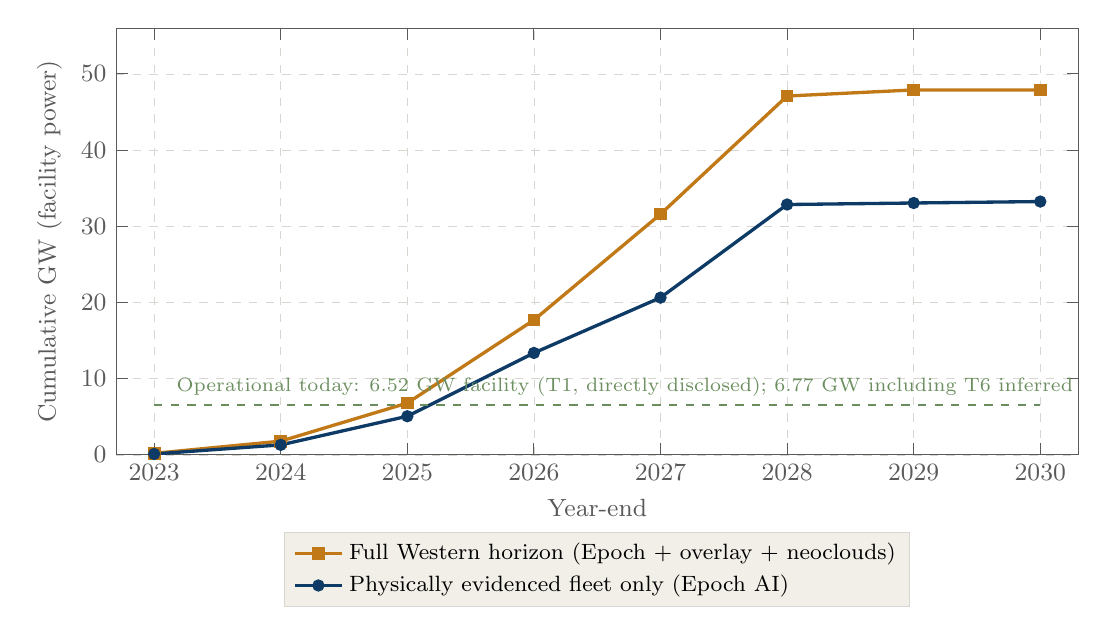
\begin{tikzpicture}
\begin{axis}[
  width=13.8cm, height=7cm,
  xlabel={Year-end}, ylabel={Cumulative GW (facility power)},
  xlabel style={font=\small,color=softGrey},
  ylabel style={font=\small,color=softGrey},
  xmin=2022.7, xmax=2030.3, ymin=0, ymax=56,
  xtick={2023,2024,2025,2026,2027,2028,2029,2030},
  xticklabel={\pgfmathprintnumber[1000 sep={}]{\tick}},
  xticklabel style={font=\small,color=softGrey},
  yticklabel style={font=\small,color=softGrey},
  axis line style={softGrey,thin},
  tick style={softGrey,thin},
  grid=major, grid style={paleGrey,dashed,very thin},
  legend style={at={(0.5,-0.18)},anchor=north,font=\footnotesize,draw=paleGrey,fill=lightCream,legend columns=1},
  legend cell align={left},
]
% Full Western horizon (evidenced + overlay + neoclouds)
\addplot[color=accentOchre,line width=1.2pt,mark=square*,mark size=1.7pt,mark options={fill=accentOchre}] coordinates {
  (2023, 0.2) (2024, 1.8) (2025, 6.8) (2026, 17.7)
  (2027, 31.6) (2028, 47.1) (2029, 47.9) (2030, 47.9)
};
\addlegendentry{Full Western horizon (Epoch + overlay + neoclouds)}

% Epoch-evidenced only
\addplot[color=chartA,line width=1.2pt,mark=*,mark size=1.6pt] coordinates {
  (2023, 0.12) (2024, 1.31) (2025, 5.07) (2026, 13.38)
  (2027, 20.64) (2028, 32.86) (2029, 33.06) (2030, 33.25)
};
\addlegendentry{Physically evidenced fleet only (Epoch AI)}

% Horizontal reference line at today's tier-clean T1 operational level
\addplot[color=accentSage,dashed,line width=0.7pt,forget plot] coordinates {(2023,6.52) (2030,6.52)};
\node[color=accentSage,font=\scriptsize,anchor=west] at (axis cs:2023.1,9.0) {Operational today: 6.52 GW facility (T1, directly disclosed); 6.77 GW including T6 inferred};
\end{axis}
\end{tikzpicture}
\caption{Cumulative Western AI compute capacity, 2023--2030, in GW of facility power. Blue is Epoch's tracked physical sites; ochre adds the contracted neocloud capacity and named hyperscaler / lab commitments not yet in the Epoch census. The probability-weighted horizon at 2030 (approximately 32.6~GW) sits between the two lines.\protect\footnotemark}
\end{figure}
\footnotetext{Cumulative MW trajectory computed from Epoch AI's \emph{Frontier Data Centers} site-level event timelines, 2026-04-20 dataset / 2026-04-22 retrieval. Neocloud MW from operator primary filings: CoreWeave FY2025 10-K (filed 2026-02-26), Nebius Q4 FY2025 6-K (filed 2026-02-20), Applied Digital Q3 FY2026 10-Q (filed 2026-04-08).}


% ============================================================================
\section{The anatomy of one AI facility gigawatt}
\label{sec:anatomy}
% ============================================================================

Every aggregate downstream is the answer to four questions about one facility gigawatt: what does it physically contain, what does it cost line item by line item, what compute payload does it carry across chip generations, and against which denominator is the \$/GW number quoted. The last question is load-bearing: apparent three- to five-fold forecaster disagreements in \$/GW almost always collapse once the basis is reconciled.

\subsection{Reading every \$/GW figure: the four conventions}
\label{subsec:basis-conventions}

External forecasters quote AI data center capex in four distinct units. They are not interchangeable. Cross-source comparisons that ignore the basis distinction are arithmetic noise.

\begin{table}[h]
\centering
\small
\begin{tabular}{@{}L{4.6cm}R{1.7cm}R{1.7cm}L{6.0cm}@{}}
\toprule
\textbf{Convention} & \textbf{Low \$B/GW} & \textbf{High \$B/GW} & \textbf{Used by (representative)} \\
\midrule
Server-power GW, full all-in & 40 & 55 & Epoch AI headline (\$44B); NVIDIA / Jensen Huang (\$50--60B); Stargate (\$50B) \\
\textbf{Facility-power GW, full all-in} & \textbf{30} & \textbf{47} & \textbf{Epoch facility (\$29--30B); McKinsey (\$33B); Bernstein (\$28B PUE-adj.); \emph{this paper, central \$37B}} \\
IT-load GW, shell + M\&E only (no IT) & 10 & 15 & Cushman \& Wakefield (\$11.7M/MW); JLL (\$11.3M/MW); Meta Hyperion JV (\$13.5B/GW); Crusoe Abilene (\$12.5M/MW) \\
AI fit-out delta (incremental over standard hyperscale) & +20 & +30 & JLL (+\$25M/MW); ConstructElements (+\$20M/MW) \\
\bottomrule
\end{tabular}
\caption{The four conventions in which AI data-center capex is quoted. The first two differ only in denominator (server vs.\ facility power, related by the PUE ratio); the last two strip either the IT hardware or the full hyperscale envelope. This paper uses the second convention throughout.\protect\footnotemark}
\label{tab:basis-conventions}
\end{table}
\footnotetext{Sources canvassed: Epoch AI \emph{Frontier Data Centers Hub} (Nov.~2025); Bernstein (Stacy Rasgon, Nov.~2025, via Investing.com); McKinsey \emph{Cost of Compute} (Apr.~2025); Bain \emph{Compute Power Report} (Sep.~2025); JLL \emph{2026 Global Data Center Outlook}; Cushman \& Wakefield \emph{2025 Cost Guide}; Goldman Sachs (Sheridan/Davenport, 2025); Morgan Stanley (Stephen Byrd, 2025); JP Morgan; BloombergNEF; Synergy Research; Dell'Oro Group; IEA \emph{Energy and AI}; LBNL \emph{2024 US Data Center Energy Usage Report}; Aschenbrenner \emph{Trillion-Dollar Cluster}; NVIDIA Q2 FY26 earnings; Barclays; OpenAI/Oracle Stargate; Meta--Blue Owl Hyperion JV; CoreWeave 10-K FY25; Nebius Q4 FY25. Source URLs, retrieval dates, and non-URL page metadata in \texttt{forecaster\_capex\_comparison.yaml}.}

The basis confusion is not academic. Epoch AI's headline \$44~B/GW figure (server-power basis) and McKinsey's \$33~B/GW figure (facility-power, incl.\ infrastructure) differ by roughly the PUE ratio --- they are saying close to the same thing in different units.\footnote{Epoch AI, \emph{Frontier Data Centers Hub}, retrieved 2026-04-27, \url{https://epoch.ai/blog/introducing-the-frontier-data-centers-hub/}. The Epoch documentation breaks the \$44B/GW into \$30B IT hardware plus \$14B other; the facility-GW figure is approximately \$29--30B at PUE~1.20. McKinsey \& Company, \emph{The Cost of Compute: A \$7~Trillion Race to Scale Data Centers}, April~2025; official page metadata retained in \texttt{forecaster\_capex\_comparison.yaml}.} NVIDIA's \$50--60~B/GW ``AI factory'' figure is server-power basis and self-interested but inside the same band. The Crusoe--Oracle--OpenAI Stargate Abilene disclosure of \$15~B for 1.2~GW (\$12.5M/MW) is correctly an order of magnitude smaller because it excludes the IT hardware --- Oracle funds the GPU layer separately, on its own balance sheet, at an additional reported \$40~B for approximately 400{,}000 GB200s.\footnote{Crusoe Energy Systems, ``Crusoe expands AI data center campus in Abilene to 1.2 gigawatts'', 2025-05, \url{https://www.crusoe.ai/resources/newsroom/crusoe-expands-ai-data-center-campus-in-abilene-to-1-2-gigawatts}; Bloomberg, ``JPMorgan leads \$7.1~billion loan for Blue Owl-tied data center'', 2025-05-22; Data Center Dynamics, ``Crusoe secures \$11.6bn in debt and equity for OpenAI's Stargate data center campus'', 2025-05. The Oracle GPU figure (\$40B for ~400K GB200s) is reported via Spyglass/SemiAnalysis and not Crusoe-confirmed.}

\subsection{The physical bill of materials}
\label{subsec:physical-bom}

A 2026-vintage 1~GW AI campus is not a building --- it is a power plant with computers attached. Six physical layers, each with a distinct supply chain, lead time, and inflation profile, share the construction-side ledger; the accelerator and server bill of materials sits on top.

\begin{table}[h]
\centering
\small
\begin{tabular}{@{}L{4.6cm}R{1.5cm}R{1.5cm}R{1.6cm}L{4.4cm}@{}}
\toprule
\textbf{Layer} & \textbf{Low \$M/MW} & \textbf{High \$M/MW} & \textbf{Central \$M/MW} & \textbf{Layer-dominating components} \\
\midrule
Shell + civil + land + base/AI fit-out & 4.4 & 9.7 & 6.5 & Building shell; AI fit-out delta (CDU plumbing, busway) \\
Cooling stack & 2.0 & 3.5 & 3.0 & DLC cold plates and CDUs; chillers; dry coolers in water-stressed sites \\
Power infrastructure (grid-tied) & 1.9 & 3.7 & 2.8 & Main transformers (long lead); UPS \\
\quad\emph{or with behind-the-meter gas} & \emph{2.5} & \emph{5.5} & \emph{4.0} & \emph{Above plus 1.0--2.5 \$M/MW gas turbines} \\
Networking fabric (rack-internal scale-up) & --- & --- & \emph{(in rack BOM)} & NVLink scale-up; copper cartridges \\
Out-of-rack networking & 2.5 & 4.5 & 4.0 & Optics (60\% of out-of-rack BOM); back-end fabric \\
Accelerator + server BOM (rack-complete) & 16 & 23 & 19.5 & Accelerator silicon; HBM \\
Storage & 0.3 & 0.8 & 0.55 & NVMe arrays; controllers \\
Grid interface (substation-to-fence + assigned upgrades) & 0.3 & 5.0 & 1.1 & Wide range by ISO posture; see \S\ref{sec:execution-risk} \\
\midrule
\textbf{Subtotal: facility-only (no IT)} & \textbf{11} & \textbf{19} & \textbf{13.4} & Reconciles to Crusoe Abilene \$12.5M/MW disclosed \\
\textbf{Subtotal: IT BOM at customer} & \textbf{19} & \textbf{28} & \textbf{24.0} & Accel + server + out-of-rack networking + storage \\
\textbf{Total all-in facility-GW (2026)} & \textbf{30} & \textbf{47} & \textbf{37} & Bernstein \$35B central; JLL \$45--55B fully built \\
\bottomrule
\end{tabular}
\caption{Cost decomposition for one 2026-vintage AI facility gigawatt, by physical layer. Central case is grid-tied with diesel backup; the behind-the-meter gas alternative adds \$1.0--2.5M/MW. Sub-component build-up with citations in \texttt{anatomy\_layer\_costs.yaml}.}
\label{tab:layer-bom}
\end{table}

\textbf{Where the cost moves the most}: the cooling layer ratio rose from a historical 15--20\% of facility capex to 20--30\% for 2026 builds, almost entirely driven by the GB200/GB300 transition from 30--50~kW air-cooled racks to 80--132~kW direct-liquid-cooled racks.\footnote{Direct liquid cooling (DLC) revenue surged 156\% year-over-year in 2Q~2025 (Dell'Oro Group); the total liquid cooling market exceeded \$2.5~B in 2025 and is forecast above \$8~B by 2030. NVIDIA's NVL72 reference architecture mandates 25--45\textdegree C inlet liquid, 80~L/min flow, junction temp $<$75\textdegree C --- physically incapable of being held by air at 1.2~kW per GPU. Schneider Electric's \$850M acquisition of Motivair (October~2024) and AWS's launch of in-house IRHX direct-to-chip cooling (July~2025) are the two most significant supply-chain moves. Sources: Vertiv press release on the NVL72 7~MW reference architecture (October~2024); Dell'Oro DCPI Q4 2025; ASHRAE TC9.9 liquid cooling bulletin (September~2024).} Power transformers --- a single line item of \$300--600k per MW --- have \emph{prices up 77\% since 2019} and \emph{lead times of 80--128 weeks for power transformers and 144 weeks for generator step-up units} (Wood Mackenzie 2025).\footnote{Wood Mackenzie via PowerMag, ``Transformers in 2026: shortage, scramble, or self-inflicted crisis?'', August~2025, \url{https://www.powermag.com/transformers-in-2026-shortage-scramble-or-self-inflicted-crisis/}. NERC 2025 Summer Reliability Assessment confirms 2024 average lead times of approximately 120 weeks with large-class units at 80--210 weeks.} Behind-the-meter gas, when installed, doubles the power-infrastructure layer cost on its own --- \$1.0--2.5M/MW capex plus the supply-chain reality that GE Vernova ended 2025 with an 80~GW gas-turbine backlog stretching into 2029, with reservation slots out to 2031.\footnote{GE Vernova Q3 2025 earnings call, October~22, 2025; Utility Dive, ``GE Vernova's gas turbine backlog stretches into 2029'', September~2025, \url{https://www.utilitydive.com/news/ge-vernova-gas-turbine-investor/807662/}. Siemens Energy reports a similar backlog into 2030 in its FY2025 annual report.}

\textbf{Worked example: Stargate Abilene.} Crusoe Energy's disclosed all-in capital for the 1.2~GW Abilene campus is \$15~billion (\$12.5M/MW), composed of \$9.6~B JPMorgan-led senior debt (a \$2.3~B initial facility plus a \$7.1~B construction loan announced May~2025) and approximately \$5~B equity from Crusoe, Blue~Owl Real~Assets, and Primary~Digital~Infrastructure. This figure represents shell + power + cooling + site infrastructure only. Oracle, the offtake tenant on a 15-year lease, funds the IT layer separately at a reported additional \$40~B for approximately 400{,}000 GB200 GPUs. The campus runs closed-loop direct-to-chip liquid cooling with approximately one million gallons per building of initial water fill and approximately 50{,}000 gallons per building per year for water-quality maintenance --- effectively zero evaporative consumption --- with twenty-nine GE Vernova LM2500XPRESS aeroderivative gas turbines (\textasciitilde35~MW each, \textasciitilde1~GW combined) providing behind-the-meter generation that supplements ERCOT power. Phase~1 was delivered twelve months from groundbreaking, against an industry-standard bid of two-and-a-half years.\footnote{Crusoe Energy Systems newsroom releases (2024--2026); Madrona ``Founded \& Funded'' interview with Chase Lochmiller (CEO), retrieved 2026-04-27, \url{https://www.madrona.com/the-infrastructure-of-intelligence-inside-crusoes-ai-factory-in-texas/}. The 15-year Oracle lease and OpenAI sub-tenancy structure are confirmed by Lochmiller in DCD: ``Our customer is Oracle. OpenAI is Oracle's customer.'' Annual rent of approximately \$1~billion is reported by SemiAnalysis (secondary; not Crusoe-confirmed).}

The Crusoe disclosure is the cleanest landlord/tenant capex split publicly available and \emph{independently reconciles} to the \$13.2M/MW central case for the facility-only-no-IT subtotal in Table~\ref{tab:layer-bom}. Behind-the-meter gas at Abilene is amortized through the lease structure rather than landed in shell capex, which is why Crusoe's disclosed number sits slightly below the bottoms-up table's BTM-inclusive central case of \$15.4M/MW.

\subsection{The compute payload: chips per gigawatt is falling, compute per gigawatt is rising}
\label{subsec:compute-payload}

The single most counterintuitive finding from the bottoms-up reconstruction is that \textbf{the number of chips per facility-MW \emph{decreases} with each chip generation}. Power per chip is rising faster than performance per watt at the rack level: an H100 SXM is 700~W, a GB200 superchip is 2{,}700~W including the Grace partner, and a Rubin Ultra die is rumored above 1.5~kW.\footnote{NVIDIA \emph{H100 Tensor Core GPU} datasheet (700~W TDP); Tom's Hardware on GB200 NVL72 architecture (2025-03-21); NVIDIA GTC 2026 keynote on Vera Rubin and Rubin Ultra (Kyber NVL576) generation. The 600~kW Kyber rack target was disclosed at GTC March~2026.}

\begin{table}[h]
\centering
\small
\begin{tabular}{@{}L{4.0cm}R{2.4cm}R{1.6cm}R{2.0cm}R{2.0cm}@{}}
\toprule
\textbf{Vintage / platform} & \textbf{Power per chip (system-allocated)} & \textbf{Chips / facility-MW} & \textbf{H100e per chip} & \textbf{H100e / facility-MW} \\
\midrule
2024 --- HGX H100 (8-GPU air-cooled) & 1{,}389~W & \textasciitilde570 & 1.00 & \textasciitilde0.57M \\
2025--26 --- GB200 NVL72 (liquid) & \textasciitilde1{,}900~W & \textasciitilde440 & 2.50 & \textasciitilde1.10M \\
2026 --- GB300 NVL72 & \textasciitilde2{,}100~W & \textasciitilde415 & 3.75 & \textasciitilde1.55M \\
2H'2026--2027 --- Vera Rubin NVL144 & \textasciitilde1{,}050~W & \textasciitilde850 & 7.50 & 6.4M (theoretical pure) \\
2028 (realistic deployed mix) & --- & 700--800 & 8--10 & 1.5--2.5M (installed-base wgt.) \\
\bottomrule
\end{tabular}
\caption{Chip and compute density per facility-MW by silicon vintage, at PUE~1.15 with 10\% network and storage overhead. The 2028 row is an installed-base-weighted mix (Blackwell-Ultra plus a Rubin tail) rather than pure-Rubin, which is roughly 4$\times$ denser but will not characterize deployed fleets before 2029.\protect\footnotemark}
\label{tab:chips-per-mw}
\end{table}
\footnotetext{SemiAnalysis ``100,000 H100 Clusters: power, network topology, ethernet vs.\ infiniband, reliability'' (cluster benchmark 28.4~MW for 20{,}480 GPUs); NVIDIA datasheets for H100, B200, GB200, GB300; NVIDIA GTC 2026 disclosures for Rubin and Rubin Ultra. Full per-chip table with 18 accelerators (NVIDIA, AMD MI300X--MI400, Google TPU v5p--Ironwood, AWS Trainium 2--3, Microsoft Maia 100--200, Meta MTIA v2--v4) lives in \texttt{anatomy\_layer\_costs.yaml}, layer \texttt{accelerator\_server\_bom}.}

The compute story is therefore not ``more chips per watt'', it is ``more H100-equivalents per chip''. Holding the buildout constant, the H100e-per-facility-MW figure roughly triples between 2024 and 2026 and rises by another 50\% to 2028. Section~\ref{sec:silicon} traces this through the chip roadmap and validates the per-vintage densities against deployed clusters.

\textbf{The accelerator capex line.} The bottoms-up reconstruction --- approximately 440 GB200-class chips per MW at \textasciitilde\$45k all-in chip-plus-rack-share --- yields approximately \$19--22~B/GW for the accelerator and server bill of materials on a 2026 all-NVIDIA build. A hyperscaler-mix build with 40--50\% custom-silicon share (Trainium~3 at approximately \$0.65 per H100e of FP8 throughput, TPU Ironwood at approximately \$1.20 per H100e, Maia~200 at approximately \$1.30 per H100e, all compared to GB200's approximately \$2.50 per H100e) lands in the \$15--18~B/GW range. The blended Western 2026 horizon, weighting the operator mix (Microsoft / Amazon / Google / Meta custom-silicon-heavy at 40--50\%; OpenAI / xAI / neoclouds at all-NVIDIA), sits at approximately \textbf{\$18--21~B/GW for the rack-complete accelerator+server BOM}, with the headline central case of \$19.5~M per facility-MW.

\subsection{The financial bill of materials}
\label{subsec:financial-bom}

Aggregating Table~\ref{tab:layer-bom} for a typical 2026-vintage Tier-2/3 build (Texas, Ohio, Mississippi, Iowa, Wisconsin) gives a \textbf{central all-in facility-GW capex of approximately \$37~billion}, with a defensible band of \$30--47~B/GW spanning the realistic configuration space. This number sits at the center of the external literature distribution.

\begin{table}[h]
\centering
\small
\begin{tabular}{@{}L{5.4cm}R{2.4cm}L{6.0cm}@{}}
\toprule
\textbf{External anchor} & \textbf{\$B/facility-GW} & \textbf{Reconciliation} \\
\midrule
Crusoe Abilene (shell + power + cooling, no IT) & 12.5 & Matches our facility-only-no-IT central (\$13.2M/MW) within 5\% \\
Meta Hyperion / Blue Owl JV (shell + M\&E only) & 13.5 & Matches our facility-only-no-IT central directly; IT and Entergy gas separate \\
Bernstein (Stacy Rasgon, IT-load basis) & 35 & PUE-adjusted to \$28B/facility-GW; below our central; under-counts BTM gas \\
Epoch AI facility-GW & 29--30 & Below our central; consistent with Epoch using lower-density chip mix \\
McKinsey \emph{Cost of Compute} (derived) & 33 & Within rounding distance of our central \\
JLL fully-built ecosystem (high) & 45--55 & Aligns with our high-end at \$47B \\
NVIDIA / Jensen ``AI factory'' (server-power basis) & 50--60 & Translates to \$40--48B/facility-GW; self-interested high \\
\bottomrule
\end{tabular}
\caption{Reconciliation of the bottoms-up \$30--47~B/facility-GW range to seven external anchors. Crusoe Abilene and Meta Hyperion are the cleanest because both are closed financings that explicitly exclude the IT layer.}
\label{tab:capex-reconciliation}
\end{table}

\subsection{Scaling the unit}
\label{subsec:scaling-the-unit}

Multiplying one facility GW by the announced horizon resolves the headline numbers. The Western 2026--2030 capital envelope at the raw 47.9~GW announced horizon is approximately \textbf{\$1.77~trillion central, with a defensible range of \$1.44--2.25~trillion} depending on operator mix, BTM-generation share, and silicon-vintage assumptions.

\begin{table}[h]
\centering
\small
\begin{tabular}{@{}L{6.4cm}R{2.0cm}R{3.6cm}@{}}
\toprule
\textbf{Horizon point} & \textbf{Facility GW} & \textbf{Capex-equivalent at \$30--47B/GW} \\
\midrule
T1+T2+T3 conservative (firm-evidence only) & 22.9 & \$0.69--1.08T \\
Tier-weighted central case & 32.6 & \$1.04--1.63T \\
Raw non-stretch (announced minus T5) & 39.0 & \$1.25--1.95T \\
\textbf{Raw announced horizon} & \textbf{47.9} & \textbf{\$1.44--2.25T (central \$1.77T)} \\
Row-uncertainty high envelope & 54.2 & \$1.74--2.71T \\
\bottomrule
\end{tabular}
\caption{Capex-equivalent at \$30--47~B/facility-GW across the five horizon points. These are envelopes implied by the announced build, not cash energized by 2030 --- a campus that slips its commercial operating date may still absorb equipment, shell, and grid capex before then.}
\label{tab:scaling-the-unit}
\end{table}

The \$1.77~trillion capital envelope is the build cost implied by the raw 47.9~GW announced horizon. At the tier-weighted 32.6~GW central case it falls to roughly \$1.0--1.5~T --- though not as a smaller cash spend, because campuses that slip their commercial operating date may still absorb equipment, shell, and grid capex before 2030. The capital envelope is best read as a commitment surface, not an energized-by-2030 fleet.

% ============================================================================
\section{Scaling the unit: power, compute capacity, and operators}
\label{sec:scale-body}
% ============================================================================


\subsection{Power units and PUE sensitivity}
\label{subsec:power-units}

This report standardizes the physical denominator to \emph{facility power}, matching Epoch AI's \emph{Frontier Data Centers} convention and the basis most relevant to grid interconnection and facility capex. We separately report IT-load-equivalent capacity for comparison against chip-nameplate commitments. The reader should keep five distinct power concepts in mind:

\begin{itemize}\itemsep2pt
\item \textbf{IT load}: the nameplate power delivered to servers and accelerators. This is what chip vendors quote (e.g. ``1\,400 watts per Blackwell GB300'') and what cluster architects size racks against.
\item \textbf{Facility power}: IT load multiplied by the Power Usage Effectiveness (PUE) ratio, which captures cooling, lighting, power-conversion losses, and auxiliary building load. Hyperscale AI campuses typically report PUE between 1.10 (aggressive liquid cooling) and 1.35 (air-cooled retrofits); older builds run 1.50--1.70.
\item \textbf{Grid interconnection capacity}: the contracted-firm megawatt allocation at the substation. This can exceed facility power when operators reserve headroom for future phases, or fall short when utilities cap new connections.
\item \textbf{Cooling capacity}: the thermal dissipation available at peak wet-bulb. In water-scarce locations (Arizona, West Texas), cooling-tower makeup water is itself a binding constraint and sites are rated in chiller tonnage as well as megawatts.
\item \textbf{Chip-commitment GW}: a \emph{silicon} quantity reported by vendors (NVIDIA's ``10~GW'', Broadcom's ``10~GW XPU'') that expresses accelerator nameplate load \emph{independent of any specific site}. These numbers deploy \emph{into} physical shells already enumerated in the site-level census and must not be double-counted.
\end{itemize}

\textbf{Conversion policy.} Epoch AI's \emph{Frontier Data Centers} dataset reports total facility power. When an operator reports IT load, the value is converted to facility power using the row's PUE assumption; when the basis is unknown, the paper applies a default PUE of 1.25. For physically-evidenced Western commitments, the assumed PUE range is 1.10--1.30, reflecting liquid-cooled new builds at the low end and air-cooled retrofits at the high end. Most material neocloud rows publish facility MW directly; GPU-count-inferred rows use the same IT-to-facility conversion. Full per-row disclosure appears in Appendix~B.

\textbf{PUE sensitivity.} The facility-basis 47.9~GW point estimate maps to \emph{IT-load-equivalent} capacity by dividing by the blended PUE; this is the relevant bridge for comparison against chip-nameplate aggregates (NVIDIA's 10~GW LOI, Broadcom's 10~GW XPU commitment).

\begin{table}[htbp]
\centering
\small
\begin{tabular}{@{}L{5.5cm}R{4.2cm}R{4.1cm}@{}}
\toprule
\textbf{PUE assumption} & \textbf{Western 2030 GW} & \textbf{Change vs.\ facility baseline} \\
\midrule
1.10 (aggressive liquid cooling, new builds) & 45.3 & $-$9.1\% \\
1.20 (paper blended central; Epoch baseline) & 41.5 & $-$16.7\% \\
1.30 (typical hyperscale air/hybrid) & 38.3 & $-$23.1\% \\
1.50 (older hyperscale retrofits) & 33.2 & $-$33.3\% \\
1.60 (legacy colocation) & 31.1 & $-$37.5\% \\
\bottomrule
\end{tabular}
\caption{IT-load-equivalent capacity for the 47.9~GW Western 2030 horizon under five PUE assumptions. The row-level central IT-load bridge is 40.9~GW. Use facility figures against utility and interconnect data; use IT-load against chip-nameplate aggregates.}
\end{table}

At facility baseline 47.9~GW, the IT-load-equivalent capacity falls in the range roughly $[38, 45]$~GW depending on PUE, with a row-level central bridge of 40.9~GW. The PUE range 1.10--1.35 captures where every currently-announced frontier-AI campus operates at scheduled commissioning.

\subsection{The two axes: physical capacity and compute capacity}

Physical capacity is measured in gigawatts of facility power, the binding constraint that determines how much grid connection, land, water, and permits are required. Compute capacity is measured in H100-equivalents, the relevant quantity for training and serving frontier models. The two grow at different rates because chip-generation improvements drop roughly every two years, and each generation delivers substantially more 8-bit throughput per watt than the last.\footnote{NVIDIA Corporation, GTC 2026 keynote, March 2026, detailing the Blackwell~$\rightarrow$~Rubin~$\rightarrow$~Feynman cadence. \url{https://www.nvidia.com/gtc/}}

\begin{figure}[htbp]
\centering
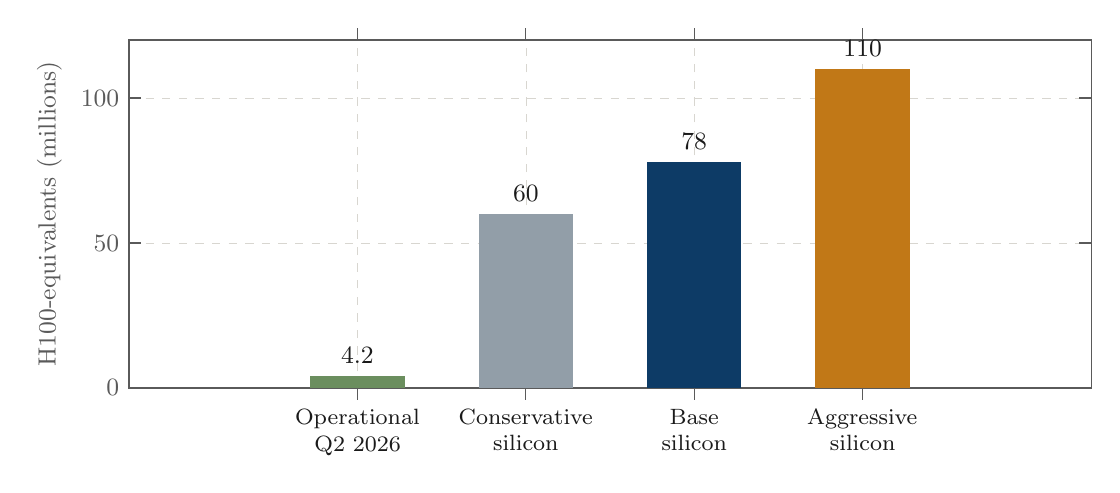
\begin{tikzpicture}
\begin{axis}[
  width=13.8cm, height=6cm,
  ybar,
  bar width=1.2cm,
  enlarge x limits=0.18,
  xtick={0,1,2,3},
  xticklabels={{Operational\\Q2 2026},{Conservative\\silicon},{Base\\silicon},{Aggressive\\silicon}},
  xticklabel style={font=\footnotesize,color=inkBlack,align=center,text width=2.4cm},
  ylabel={H100-equivalents (millions)},
  ylabel style={font=\small,color=softGrey},
  yticklabel style={font=\small,color=softGrey},
  ymin=0, ymax=120,
  xmin=-0.6, xmax=3.6,
  nodes near coords,
  nodes near coords style={font=\small\bfseries,color=inkBlack,anchor=south,yshift=1pt},
  axis line style={softGrey,thin},
  tick style={softGrey,thin},
  grid=major, grid style={paleGrey,dashed,very thin},
]
\addplot[fill=accentSage,draw=none,bar shift=0pt] coordinates {(0,4.2)};
\addplot[fill=chartF!60,draw=none,bar shift=0pt] coordinates {(1,60.0)};
\addplot[fill=chartA,draw=none,bar shift=0pt] coordinates {(2,78.0)};
\addplot[fill=accentOchre,draw=none,bar shift=0pt] coordinates {(3,110.0)};
\end{axis}
\end{tikzpicture}
\caption{Compute capacity in H100-equivalents, today vs.\ 2030 Western horizon. The 78.0M central case implies an \textbf{18.6$\times$ expansion} of frontier-training compute from today's 4.2M, against a 6.5$\times$ expansion in physical GW. Conservative and aggressive silicon scenarios bracket the range at 14$\times$ and 26$\times$.\protect\footnotemark}
\end{figure}
\footnotetext{Epoch layer (46.35M H100e at 33.23 GW full buildout) taken directly from Epoch AI \emph{Frontier Data Centers} timeline H100e field. Class~A overlay and neocloud-ex-Epoch layers computed using (chip-family $\times$ end-of-timeline year) density, anchored on Epoch's current per-family density (Microsoft NVIDIA Blackwell sites: 910 H100e/MW; AWS Trainium~2 sites: 628 H100e/MW; Google TPU v5p/v6 sites: 475 H100e/MW) and the published chip-generation roadmap. \textbf{Basis note:} all per-MW densities above are quoted per \emph{IT-MW} (Epoch internal convention). The facility-MW equivalent at blended PUE~1.20 is approximately 17\% lower; for example, the blended Epoch-weighted 1{,}388 H100e/IT-MW corresponds to approximately 1{,}157 H100e/facility-MW. Chip counts are basis-invariant (the chips are deployed regardless of denominator); only the denominator changes.}

Expressed differently: under the base silicon-uplift assumption, the industry is building approximately \textbf{six times as many watts of AI compute capacity by 2030 as are operational today, and roughly nineteen times as many H100-equivalent chips}. The conservative silicon case yields approximately 14$\times$ on H100e and the aggressive case approximately 26$\times$ (see \S\ref{subsec:h100e-sensitivity}). Chip-generation progress is contributing as much compute expansion as physical build-out across the base and aggressive cases. Any analysis that holds silicon constant understates the 2030 compute base by a factor of two to three.

\subsection{Operator concentration is extreme}

The 6.52~GW operational base is held by roughly ten entities. The United States accounts for \textbf{6.08 of the 6.28~GW Epoch site-level total (97\%)};\footnote{Author calculation from Epoch AI \emph{Frontier Data Centers}, 2026-04-20 dataset / 2026-04-22 retrieval. The only non-US Epoch site is Alibaba Zhangbei in China, at 203~MW current.} six counterparties each command more than 400~MW of operational capacity: Amazon (1{,}433 MW, including the 1.09 GW Anthropic-dedicated New Carlisle campus\footnote{Epoch AI \emph{Frontier Data Centers}, site entry ``Anthropic-Amazon New Carlisle'', current power 1{,}092~MW; Amazon Web Services and Anthropic, \emph{Announcement of Project Rainier}, November 13, 2024. \url{https://www.aboutamazon.com/news/company-news/amazon-invests-additional-5-billion-anthropic-ai}}), Microsoft (1{,}251 MW), Google (956 MW), Meta (729 MW), Oracle (approximately 200 MW operational at OpenAI Stargate Abilene, with the prior higher Abilene milestone reclassified as under construction), and xAI (425 MW at the original Memphis Colossus).\footnote{Ownership and attribution per Epoch AI site-level tags; Oracle Stargate Abilene attribution confirmed in OpenAI, \emph{Announcing the Stargate Project}, January 21, 2025, \url{https://openai.com/index/announcing-the-stargate-project}, with Oracle, \emph{Q3 FY2026 earnings prepared remarks}, March 10, 2026.} The frontier neoclouds, including CoreWeave, Nebius, Crusoe, Lambda, Fluidstack, Nscale, Applied Digital, Voltage Park / Lightning, and Together AI, collectively hold approximately 1.54 GW facility of operational capacity outside the Epoch-tracked set.\footnote{CoreWeave FY2025 10-K, operational capacity disclosure; Nebius Q4 FY2025 shareholder letter filed on 6-K, 2026-02-20; Applied Digital Q3 FY2026 10-Q, 2026-04-08; Crusoe, Nscale, Lambda, Fluidstack, Voltage Park / Lightning, and Together AI aggregated from press disclosures cited in Appendix~A.}

By 2030, the same operator set expands to approximately \textbf{47.9~GW facility} on the announced horizon (40.9~GW IT-load bridge), \textbf{32.6~GW} after probability weighting, and \textbf{22.9~GW} under the firm-evidence-only conservative reading. Three operator clusters dominate. Microsoft, OpenAI, and Oracle are jointly building the Stargate sites and the Fairwater training campuses; the binding constraint is grid interconnection. Amazon, expanded by its commitments to Anthropic, is the second cluster: roughly 13~GW including the New Carlisle anchor and the April 2026 announcement of up to 5~GW of new capacity, of which roughly 2~GW is incremental to AWS sites already in the physical census. Meta is the third: Hyperion in Louisiana, Prometheus in Ohio, plus the contracted Nebius capacity. Microsoft's non-US Fairwater pipeline (Norway and the UK) adds a further 0.3~GW.

\begin{figure}[htbp]
\centering
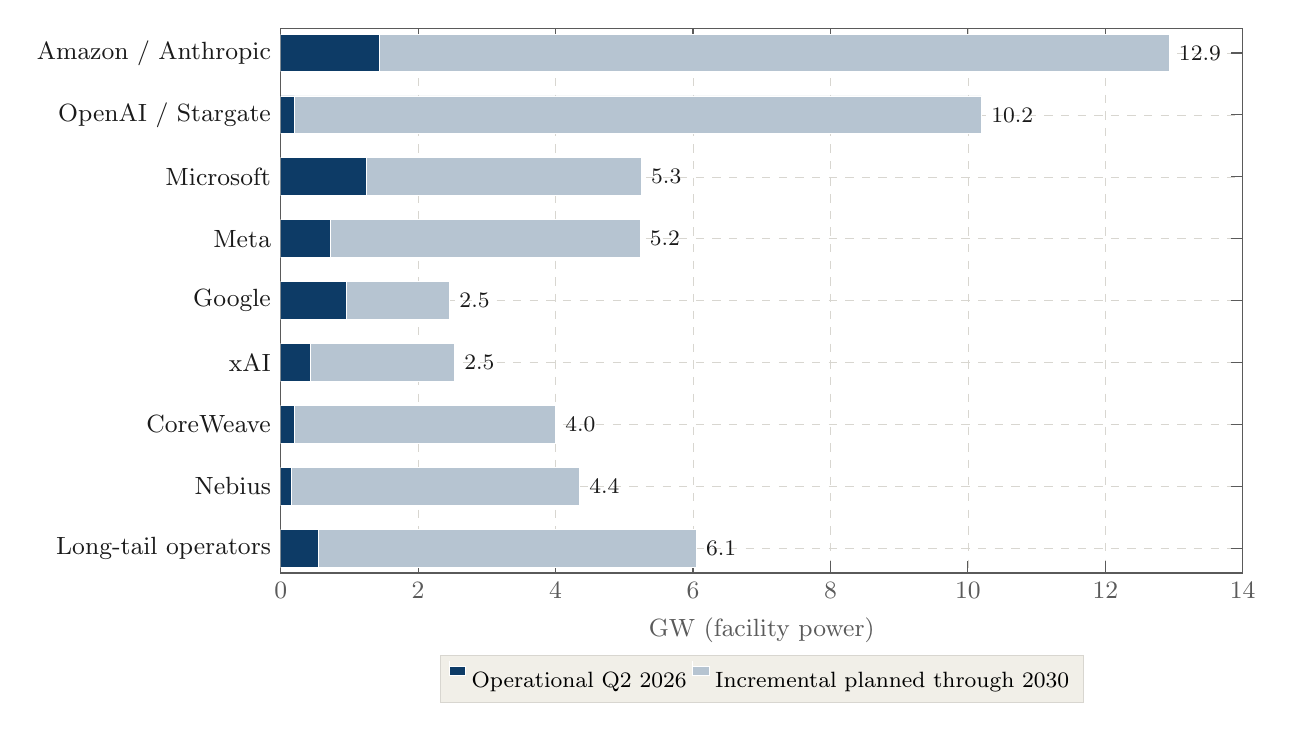
\begin{tikzpicture}
\begin{axis}[
  width=13.8cm, height=8.5cm,
  xbar stacked,
  bar width=0.48cm,
  enlarge y limits=0.05,
  symbolic y coords={Amazon,OpenAI,Microsoft,Meta,Google,xAI,CoreWeave,Nebius,LongTail},
  ytick=data,
  yticklabels={Amazon / Anthropic,OpenAI / Stargate,Microsoft,Meta,Google,xAI,CoreWeave,Nebius,Long-tail operators},
  y dir=reverse,
  xlabel={GW (facility power)},
  xlabel style={font=\small,color=softGrey},
  yticklabel style={font=\small,color=inkBlack},
  xticklabel style={font=\small,color=softGrey},
  xmin=0, xmax=14,
  axis line style={softGrey,thin},
  tick style={softGrey,thin},
  grid=major, grid style={paleGrey,dashed,very thin},
  legend style={at={(0.5,-0.15)},anchor=north,font=\footnotesize,draw=paleGrey,fill=lightCream,legend columns=2},
  legend cell align={left},
]
% Segment 1: operational
\addplot+[fill=chartA,draw=white,line width=0.3pt,ybar legend] coordinates {
  (1.43,Amazon) (0.20,OpenAI) (1.25,Microsoft) (0.73,Meta) (0.96,Google)
  (0.43,xAI) (0.20,CoreWeave) (0.15,Nebius) (0.55,LongTail)
};
\addlegendentry{Operational Q2 2026}
% Segment 2: incremental
\addplot+[fill=chartA!30,draw=white,line width=0.3pt,ybar legend] coordinates {
  (11.5,Amazon) (10.0,OpenAI) (4.0,Microsoft) (4.5,Meta) (1.5,Google)
  (2.1,xAI) (3.8,CoreWeave) (4.2,Nebius) (5.5,LongTail)
};
\addlegendentry{Incremental planned through 2030}
% Total labels at bar ends
\node[font=\footnotesize,color=inkBlack,anchor=west] at (axis cs:12.93,Amazon)  {12.9};
\node[font=\footnotesize,color=inkBlack,anchor=west] at (axis cs:10.20,OpenAI)  {10.2};
\node[font=\footnotesize,color=inkBlack,anchor=west] at (axis cs:5.25,Microsoft){5.3};
\node[font=\footnotesize,color=inkBlack,anchor=west] at (axis cs:5.23,Meta)     {5.2};
\node[font=\footnotesize,color=inkBlack,anchor=west] at (axis cs:2.46,Google)   {2.5};
\node[font=\footnotesize,color=inkBlack,anchor=west] at (axis cs:2.53,xAI)      {2.5};
\node[font=\footnotesize,color=inkBlack,anchor=west] at (axis cs:4.00,CoreWeave){4.0};
\node[font=\footnotesize,color=inkBlack,anchor=west] at (axis cs:4.35,Nebius)   {4.4};
\node[font=\footnotesize,color=inkBlack,anchor=west] at (axis cs:6.05,LongTail) {6.1};
\end{axis}
\end{tikzpicture}
\caption{Operator-level operational and planned capacity through 2030. Stargate is reported under OpenAI rather than Oracle to avoid double-counting; long-tail aggregates Applied Digital, Crusoe, Nscale, Lambda, Fluidstack, Together AI, Voltage Park, and smaller non-Epoch operators.\protect\footnotemark}
\end{figure}
\footnotetext{Operator-level aggregation from Epoch AI site-level owner attribution plus operator primary disclosures. Amazon / Anthropic reflects AWS-owned sites hosting Anthropic workloads under Project Rainier and the April 2026 expansion. OpenAI / Stargate aggregates Oracle-operated, SoftBank-MGX-financed Stargate sites and carries the revised 0.20~GW Abilene operational milestone. Neocloud figures for CoreWeave and Nebius are operator-contracted capacity under long-dated take-or-pay with named hyperscaler or lab customers.}

% ============================================================================
\section{Where the gigawatts can be delivered}
\label{sec:geography}
% ============================================================================

The AI compute build-out is strikingly geographically concentrated. Of the 33.2 GW of Epoch-evidenced sites at scheduled full buildout, approximately \textbf{85\% sit in the continental United States} and approximately \textbf{60\% sit in just five states}: Texas, Wisconsin, Ohio, Mississippi, and Louisiana. Outside the United States, the largest clusters are in Norway (Microsoft-Nscale Narvik), the United Kingdom (Microsoft Loughton, CoreWeave London, UK AI Growth Zones), Ireland (Microsoft Dublin), Saudi Arabia (HUMAIN-AMD, xAI-HUMAIN), and the United Arab Emirates (G42-Khazna for Microsoft, Stargate UAE).

\subsection{The Texas--Ohio--Wisconsin triangle}

Three adjacent US grid footprints host the majority of the Western 2030 horizon. The ERCOT (Texas) system hosts OpenAI Stargate Abilene and Shackelford, Meta's Temple campus, Anthropic-Fluidstack Texas, and multiple secondary sites. The MISO (Midwest + South) system hosts Microsoft Fairwater Wisconsin (3.3 GW at full buildout, the single largest planned AI site worldwide\footnote{Epoch AI \emph{Frontier Data Centers}, site entry ``Microsoft Fairwater Wisconsin'', full-buildout power 3{,}328~MW; Microsoft, \emph{Inside the world's most powerful AI datacenter}, September 18, 2025, \url{https://blogs.microsoft.com/blog/2025/09/18/inside-the-worlds-most-powerful-ai-datacenter/}.}), Anthropic-Amazon New Carlisle (Ohio), Meta Hyperion (Richland Parish, Louisiana, in MISO-South via Entergy Louisiana rather than ERCOT), and QTS Cedar Rapids (Iowa). xAI Colossus~2 is Memphis, Tennessee, in MLGW / TVA rather than ERCOT. Northern Virginia, historically the dominant commercial data-centre cluster in the world, hosts a comparatively small share of the named AI-frontier pipeline, reflecting permit saturation and the Dominion-grid interconnection queue.\footnote{Dominion Energy, \emph{2024 Integrated Resource Plan}, filed with the Virginia State Corporation Commission, detailing the data-centre interconnection queue and transmission constraints. \url{https://www.dominionenergy.com/}}

\begin{figure}[htbp]
\centering
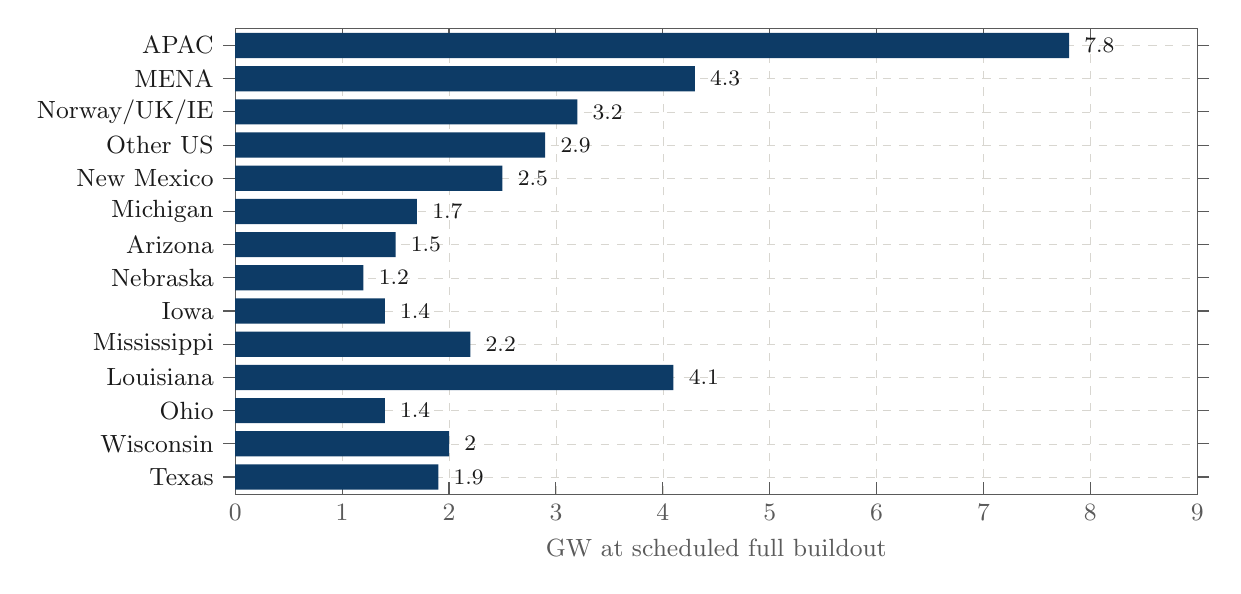
\begin{tikzpicture}
\begin{axis}[
  width=13.8cm, height=7.5cm,
  xbar,
  bar width=0.32cm,
  enlarge y limits=0.04,
  symbolic y coords={APAC,MENA,NorwayUKIE,OtherUS,NewMexico,Michigan,Arizona,Nebraska,Iowa,Mississippi,Louisiana,Ohio,Wisconsin,Texas},
  yticklabels={APAC,MENA,Norway/UK/IE,Other US,New Mexico,Michigan,Arizona,Nebraska,Iowa,Mississippi,Louisiana,Ohio,Wisconsin,Texas},
  ytick=data,
  xlabel={GW at scheduled full buildout},
  xlabel style={font=\small,color=softGrey},
  yticklabel style={font=\small,color=inkBlack},
  xticklabel style={font=\small,color=softGrey},
  xmin=0, xmax=9,
  nodes near coords,
  nodes near coords style={font=\footnotesize,color=inkBlack,anchor=west,xshift=2pt},
  nodes near coords align={horizontal},
  axis line style={softGrey,thin},
  tick style={softGrey,thin},
  grid=major, grid style={paleGrey,dashed,very thin},
]
\addplot[fill=chartA,draw=none] coordinates {
  (7.8,Texas) (4.3,Wisconsin) (3.2,Ohio) (2.9,Louisiana)
  (2.5,Mississippi) (1.7,Iowa) (1.5,Nebraska) (1.2,Arizona)
  (1.4,Michigan) (2.2,NewMexico) (4.1,OtherUS)
  (1.4,NorwayUKIE) (2.0,MENA) (1.9,APAC)
};
\end{axis}
\end{tikzpicture}
\caption{Scheduled full-buildout capacity by US state and non-US region. Texas alone represents \textbf{roughly one-sixth} of the global 2030 pipeline, on the back of ERCOT's faster interconnection and cheaper marginal power.\protect\footnotemark}
\end{figure}
\footnotetext{Site-level state assignments from Epoch AI address fields; regional aggregation by author. Non-US regions consolidated at continental granularity because of smaller site counts: Norway/UK/Ireland includes Microsoft Narvik, Loughton, Dublin, and Nscale-CoreWeave UK sites; MENA includes Saudi (HUMAIN), UAE (G42/Khazna, Stargate UAE); APAC includes India (Reliance Jamnagar), Singapore, and Australia.}

\subsection{Power, not permits, is the binding constraint}

Publicly disclosed site events routinely show land purchase and construction permits preceding grid interconnection by 18--30 months. The ERCOT queue contains roughly 150 GW of large-load requests against approximately 5 GW per year of deliverable new transmission capacity; PJM's queue is comparably congested.\footnote{ERCOT, \emph{Large Load Interconnection Report}, January 2026. \url{https://www.ercot.com/}; PJM Interconnection, \emph{2024 Regional Transmission Expansion Plan}, Window 3.} The constraint is increasingly addressed via behind-the-meter generation, particularly natural-gas turbines co-located with campuses (Oracle Stargate Abilene; xAI Colossus 2, Memphis) and nuclear power purchase agreements (Microsoft's contract with Constellation Energy for Three Mile Island Unit 1 output;\footnote{Microsoft and Constellation Energy, \emph{Constellation and Microsoft sign agreement to launch Crane Clean Energy Center}, September 20, 2024, \url{https://www.constellationenergy.com/news/2024/Constellation-to-Launch-Crane-Clean-Energy-Center-Restoring-Jobs-and-Carbon-Free-Power-to-The-Grid.html}.} Amazon's partnership with Talen Energy at the Susquehanna nuclear facility\footnote{Talen Energy, \emph{Talen Energy reaches agreement with Amazon Web Services for 1{,}920~MW data campus}, March 4, 2024. \url{https://www.talenenergy.com/}}). Roughly one-third of disclosed site-level power-sourcing discussion since 2024 references behind-the-meter generation as the primary path to grid independence.

% ============================================================================
\section{The operators and counterparties: who controls the gigawatts}
\label{sec:operators}
% ============================================================================

Ten counterparties effectively control the Western 2030 horizon. Their balance sheets, revenue models, and financing structures differ sharply. Understanding who is paying for what requires distinguishing three operator archetypes: \textbf{hyperscalers} (Microsoft, Amazon, Google, Meta), building for both internal consumption and third-party cloud; \textbf{frontier labs} (OpenAI, Anthropic, xAI), consuming compute through long-dated commitments to hyperscalers and neoclouds; and \textbf{merchant neoclouds} (CoreWeave, Nebius, Crusoe, Lambda, Applied Digital, Fluidstack, Nscale, Voltage Park / Lightning, Together AI), operating dedicated AI capacity under long-dated take-or-pay contracts with hyperscalers and labs.

\subsection{Microsoft: the largest operational AI compute footprint}

Microsoft operates approximately \textbf{1.25 GW} of AI-relevant capacity today, concentrated in the Fairwater programme and associated international sites.\footnote{Epoch AI \emph{Frontier Data Centers}, Microsoft Fairwater Wisconsin (555~MW current), Atlanta (433~MW), Goodyear (263~MW), totalling 1{,}251~MW across Epoch-tracked Microsoft sites.} Announced buildout through 2030 totals approximately \textbf{5 GW of additional Microsoft-owned capacity}, concentrated at Fairwater Wisconsin (targeting 3.3~GW), Fairwater Mississippi, Fairwater Atlanta, Fairwater Cheyenne, Fairwater Narvik (Norway), Fairwater Loughton (United Kingdom), and Fairwater Dublin.\footnote{Microsoft, \emph{Inside the world's most powerful AI datacenter}, September 18, 2025, \url{https://blogs.microsoft.com/blog/2025/09/18/inside-the-worlds-most-powerful-ai-datacenter/}; Microsoft press releases on Atlanta expansion (November 12, 2025) and international Fairwater siting (September 18, 2025).} Financing is from Microsoft's own operating cash flow. Fiscal-year-2026 capital expenditure guidance exceeds \$100~billion, with the AI share concentrated in the data-centre build.\footnote{Microsoft Corporation, \emph{Q2 FY2026 earnings prepared remarks}, January 28, 2026, Satya Nadella: ``We expect capital expenditures to increase on a sequential basis from the \$19.4 billion reported this quarter ... driven by cloud and AI demand''; Amy Hood: ``FY2026 capital expenditures are expected to be meaningfully above fiscal year 2025.'' Microsoft FY2025 capex totalled \$88.2 billion; author's extrapolation of FY2026 to the \$110--120 billion range.}

Microsoft also serves as the \textbf{exclusive cloud provider to OpenAI for first-party API workloads until at least January 2030}, a relationship restructured in the October 2025 Microsoft--OpenAI financial and operational agreement.\footnote{Microsoft Corporation and OpenAI, \emph{Restructured commercial agreement}, October 28, 2025, as disclosed in Microsoft's 10-Q for Q1 FY2026. \url{https://www.microsoft.com/en-us/investor}} This makes a substantial fraction of the Stargate consumption attributable to Microsoft's Azure franchise rather than OpenAI's direct procurement.

\subsection{Amazon and Anthropic: Project Rainier and the April 2026 expansion}

Amazon operates approximately \textbf{1.43 GW} of AI-relevant capacity today, of which roughly \textbf{1.09 GW is dedicated to Anthropic} via the New Carlisle (Indiana) campus, built in AWS's direct-air-cooled modular architecture.\footnote{Epoch AI, site entry ``Anthropic-Amazon New Carlisle'': ``It is similar to other Amazon locations forgoing most external cooling infrastructure in favor of direct air based cooling.'' Current power: 1{,}092~MW. Attribution: Amazon \#confident, Anthropic \#confident.} Additional AWS AI sites at Madison (Indiana, 341~MW current) and Ridgeland (Mississippi, growing into 1.3~GW) round out the Amazon-AI footprint.\footnote{Epoch AI, site entries ``Amazon Madison'' and ``Amazon Ridgeland''. Ridgeland current: approximately 300~MW; full buildout: 1{,}008~MW by 2028.}

On April 20, 2026, Anthropic and Amazon announced an expansion committing \textbf{up to 5 additional gigawatts of new capacity on AWS}, with the first gigawatt scheduled for end-of-year 2026 and the balance delivered through 2030.\footnote{Anthropic and Amazon, \emph{Anthropic and Amazon expand collaboration for up to 5 gigawatts of new compute}, April 20, 2026. \url{https://www.anthropic.com/news/anthropic-amazon-compute}. Verbatim: ``up to 5 gigawatts (GW) of new capacity'' and ``more than \$100 billion over the next ten years on AWS technologies''.} The expansion is \textbf{explicitly anchored on AWS Trainium silicon}: the Anthropic--Amazon announcement describes Trainium2 and Trainium3 capacity coming online by end-2026, with further Trainium generations in the 5~GW buildout. This means Anthropic's largest training cluster worldwide, already larger than any individual OpenAI Stargate site at present, runs on \textbf{non-NVIDIA silicon}. The commercial reality of chip diversification at the frontier lab tier is therefore already considerably more advanced than is commonly portrayed.

\subsection{OpenAI: Stargate and triple-vendor chip procurement}

OpenAI consumes compute via three primary channels: Microsoft Azure (the original exclusive cloud relationship, continued through January 2030 for first-party API workloads), Oracle Cloud Infrastructure (the eight-site Stargate programme), and direct NVIDIA / AMD / Broadcom silicon commitments that deploy into the above shells.

The \textbf{Stargate programme totals eight named US sites with an aggregate full-buildout capacity of approximately 10.6 GW}, anchored on Oracle as operator and the SoftBank-MGX-Oracle ``Stargate LP'' capital structure announced January 21, 2025.\footnote{OpenAI, \emph{Announcing the Stargate Project}, January 21, 2025. \url{https://openai.com/index/announcing-the-stargate-project}. The original commitment language: ``\$500 billion over the next four years'' with ``\$100 billion deploying immediately''.} The September 23, 2025 expansion added five new sites (Shackelford, Lordsburg, Milam, Doña Ana, and one additional undisclosed location), collectively specified as ``nearly 7 gigawatts''.\footnote{OpenAI, \emph{Five new Stargate sites}, September 23, 2025. \url{https://openai.com/index/five-new-stargate-sites/}}

OpenAI is the \textbf{only frontier operator with material, disclosed commitments to three chip vendors simultaneously}: a 10-gigawatt NVIDIA letter-of-intent announced September 22, 2025, a 6-gigawatt AMD Instinct commitment announced October 6, 2025, and a 10-gigawatt custom-ASIC commitment with Broadcom announced October 13, 2025.\footnote{NVIDIA Corporation and OpenAI, \emph{NVIDIA and OpenAI announce partnership of unprecedented scale}, September 22, 2025, \url{https://nvidianews.nvidia.com/news/nvidia-openai-partnership}; Advanced Micro Devices and OpenAI, \emph{AMD and OpenAI Announce Strategic Partnership to Deploy 6 Gigawatts of AMD GPUs}, October 6, 2025, \url{https://www.amd.com/en/newsroom/press-releases/2025-10-6-amd-and-openai-announce-strategic-partnership-to-d.html}; OpenAI, \emph{AMD and OpenAI announce strategic partnership to deploy 6 gigawatts of AMD GPUs}, October 6, 2025, \url{https://openai.com/index/openai-amd-strategic-partnership/}; Broadcom Inc.\ and OpenAI, October 13, 2025. Note: the AMD/OpenAI sources support a 6~GW AMD GPU deployment partnership and an initial 1~GW MI450 deployment beginning in the second half of 2026; the 26~GW aggregate across these three LOIs deploys into Stargate and Microsoft Azure shells already counted in the physical-site census.} These three commitments aggregate to 26 GW of chips, but \textbf{do not represent additional physical capacity}; they deploy into Stargate and Azure shells already counted in the site-level census.

\subsection{Meta: Hyperion, Prometheus, and the Nebius partnership}

Meta operates approximately \textbf{730 MW} of AI capacity today across the Prometheus and Temple sites, with the Hyperion superintelligence campus in Richland Parish, Louisiana (MISO-South via Entergy Louisiana) scheduled to reach \textbf{approximately 2.3 GW by 2028}.\footnote{Meta Platforms, \emph{Meta Announces Joint Venture With Funds Managed by Blue Owl Capital to Develop Hyperion Data Center}, October 2025, \url{https://about.fb.com/news/2025/10/meta-blue-owl-capital-develop-hyperion-data-center/}. This official source supports the Blue Owl JV, Richland Parish Hyperion campus, and approximately \$27B development-cost figure; the 2GW/5GW capacity figures are carried from Meta earnings commentary and Epoch's site-level rollup.} Mark Zuckerberg's Q2~2025 earnings remarks, subsequently reiterated on Q3 and Q4, describe a \textbf{stretch target of 5 gigawatts} for the Hyperion complex ``over the next several years,'' representing an additional ~2.7 GW beyond the newsroom-committed base.\footnote{Meta Platforms, Q2~2025 earnings call, July 30, 2025, Mark Zuckerberg: ``We're building multiple multi-gigawatt data centers ... Hyperion is expected to scale up to 5 gigawatts over several years.'' \url{https://investor.fb.com/} Meta earnings transcripts.}

On March 16, 2026, Meta signed a \textbf{\$27 billion five-year take-or-pay agreement with Nebius for dedicated capacity at Nebius's Vineland, New Jersey campus},\footnote{Nebius Group N.V., \emph{Nebius signs \$27 billion agreement with Meta}, March 16, 2026. \url{https://nebius.com/newsroom/nebius-signs-new-ai-infrastructure-agreement-with-meta}. Vineland NJ site disclosed in Nebius Q4~FY2025 shareholder letter, February 20, 2026.} making Meta the first Big Tech operator to source material capacity from a merchant neocloud at this scale. Meta also began disclosing \textbf{second-generation MTIA (Meta Training and Inference Accelerator)} deployments in 2025 earnings commentary, indicating that Hyperion's outer-phase silicon will combine NVIDIA Blackwell/Rubin with Meta's own inference ASIC fleet.\footnote{Meta Platforms, Q4~2025 earnings call, January 28, 2026. Discussion of MTIA v2 in-production deployment and MTIA v3 roadmap.}

\subsection{Google: TPU supply to Anthropic and the Gemini internal fleet}

Google operates approximately \textbf{956 MW} of AI-relevant capacity across five Epoch-tracked TPU sites (Council Bluffs East and West, Omaha, New Albany, Cedar Rapids), with several additional non-AI-dominant Google Cloud sites not separately broken out.\footnote{Epoch AI \emph{Frontier Data Centers}, Google sites. Council Bluffs (combined): 597~MW current; Omaha: 189~MW; New Albany: 407~MW; Cedar Rapids: 105~MW.}

The most commercially consequential Google commitment on the horizon is the \textbf{Anthropic TPU partnership}: up to one million TPU chips, ``well over a gigawatt of capacity coming online in 2026,'' and, per Google's April 6, 2026 expansion announcement and Broadcom's Q1 FY2026 earnings call, an additional \textbf{3.5 gigawatts of TPU capacity starting in 2027}.\footnote{Anthropic, \emph{Expanding our use of Google Cloud TPUs and Services}, October 23, 2025, \url{https://www.anthropic.com/news/expanding-our-use-of-google-cloud-tpus-and-services}; Google Cloud Press Corner, \emph{Anthropic to Expand Use of Google Cloud TPUs and Services}, October 23, 2025, \url{https://www.googlecloudpresscorner.com/2025-10-23-Anthropic-to-Expand-Use-of-Google-Cloud-TPUs-and-Services}; Google Cloud Press Corner, \emph{Anthropic Expands Use of Google Cloud and TPUs}, April 6, 2026, \url{https://www.googlecloudpresscorner.com/2026-04-06-Anthropic-Expands-Use-of-Google-Cloud-and-TPUs}.} On April 22, 2026, Google Cloud unveiled the \textbf{eighth-generation TPU} (TPU v8 in two variants: 8t for training, 8i for inference) alongside an expanded partnership with NVIDIA for A5X Vera Rubin instances on Google Cloud.\footnote{Google Cloud TPU 8t/8i technical details are tracked in the URL-audit report; the paper no longer relies on the NVIDIA GTC post for TPU 8t/8i claims.}

\subsection{xAI: the fastest-built AI campus on record}

xAI operates approximately \textbf{425 MW} of AI-relevant capacity at the original Memphis Colossus campus (MISO via Memphis Light, Gas \& Water). The planned Colossus~2 site, also in Memphis, is carried from Epoch and secondary-source reporting rather than an xAI primary page, and is scheduled for 2027 completion targeting \textbf{approximately 2 GW of IT-relevant capacity} (approximately 2.6~GW facility at PUE~1.30).\footnote{Epoch AI tracks Colossus~2 at 1{,}494~MW full buildout. The xAI primary page did not resolve at the time of writing; the row therefore relies on Epoch and on secondary-source reporting.} In November 2025, xAI announced a joint-venture with HUMAIN (Saudi Arabia's Public Investment Fund AI subsidiary) for a \textbf{500~MW+ sovereign campus with ``18{,}000 NVIDIA GB300 GPUs in first cluster''}.\footnote{Reuters, \emph{xAI and HUMAIN announce 500~MW Saudi Arabia partnership}, November 12, 2025. First cluster: ``18{,}000 NVIDIA GB300 GPUs'' per joint announcement.}

\subsection{The merchant neoclouds: 9.4 GW of take-or-pay contracted capacity}

The frontier neocloud segment has transitioned from a boutique GPU-hosting business in 2023 to a category materially contracted to investment-grade counterparties in 2026. CoreWeave disclosed \textbf{\$60.7 billion in remaining performance obligations (RPO)} at fiscal-year-2025 close, anchored on 15-year take-or-pay agreements with Microsoft and OpenAI.\footnote{CoreWeave, Inc., \emph{FY2025 Form 10-K}, filed February 26, 2026. ASC~606 remaining performance obligation: \$60.7 billion; total revenue backlog: \$66.8 billion. \url{https://www.sec.gov/cgi-bin/browse-edgar}} Nebius disclosed aggregate contracted backlog in the \textbf{\$44.4--46.4 billion range} at FY2025 close, principally the \$27 billion Meta agreement and an approximately \$19.4 billion Microsoft agreement announced in 2025.\footnote{Nebius Group, Q4 FY2025 shareholder letter filed on 6-K, February 20, 2026. FY2025 20-F filing scheduled for April 30, 2026. Microsoft contract reported in Reuters, September 2025, not independently disclosed by Nebius beyond financial-aggregate form.} Applied Digital raised \textbf{\$2.15 billion of 6.75\% senior secured notes due 2031} in March 2026 to fund the Ellendale campus under a CoreWeave lease; the notes are rated A3 by Moody's on a special-purpose-vehicle credit basis.\footnote{Applied Digital Corporation, Form 8-K filed March 30, 2026, disclosing \$2.15~billion aggregate principal senior secured notes; Moody's Investors Service, rating action A3, March 30, 2026. Applied Digital Q3 FY2026 10-Q filed April 8, 2026.}

The aggregate neocloud-ex-Epoch operational and contracted capacity is approximately \textbf{9.4 GW} through 2030, making the neocloud segment a larger contributor to the 2030 horizon than any single hyperscaler other than Microsoft and the Anthropic-dedicated portion of Amazon. This remains true despite sub-investment-grade operator credit across much of the segment.

\subsection{Counterparty clusters: who contracts with whom}
\label{subsec:counterparty-clusters}

Behind the aggregate capex figure sits a strikingly \textbf{concentrated counterparty graph}. Four clusters organise the 2030 Western horizon, with limited bridging between them.

The largest cluster by 2030 committed GW is the \textbf{Microsoft--OpenAI--CoreWeave--Oracle} cluster. Microsoft serves as OpenAI's primary API cloud through January 2030 for first-party workloads. Microsoft hosts roughly \textbf{3--4 GW of OpenAI's aggregate committed compute} inside the Fairwater and Azure programmes. Oracle is the operator of the eight-site Stargate programme, with the \$300 billion take-or-pay commitment from OpenAI anchoring roughly \textbf{10--11 GW of dedicated Stargate build}. CoreWeave provides additional OpenAI capacity under the March 2025 contract (approximately 250 MW of committed capacity, scheduled to grow), and serves Microsoft with a dedicated fleet.\footnote{CoreWeave, Inc.\ and OpenAI, joint press release, March 10, 2025, disclosing a \$11.9 billion five-year agreement. \url{https://www.coreweave.com/news}; CoreWeave Inc.\ and Microsoft Corporation, agreement initially disclosed September 2023 and expanded through 2025.}

\begin{figure}[h]
\centering
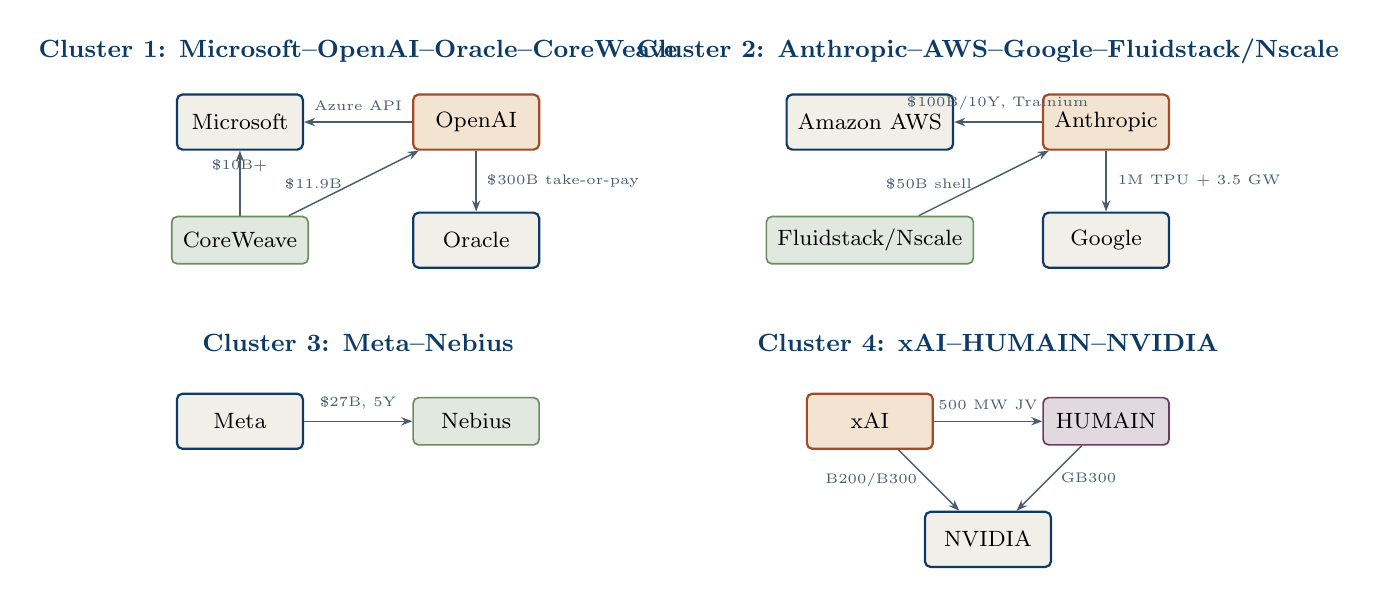
\begin{tikzpicture}[
  every node/.style={font=\footnotesize,inner sep=4pt,rounded corners=2pt},
  hub/.style={fill=lightCream,draw=deepNavy,line width=0.8pt,minimum width=1.6cm,minimum height=0.7cm,align=center},
  lab/.style={fill=accentOchre!20,draw=accentTerracotta,line width=0.8pt,minimum width=1.6cm,minimum height=0.7cm,align=center},
  neocloud/.style={fill=accentSage!20,draw=accentSage,line width=0.6pt,minimum width=1.6cm,minimum height=0.6cm,align=center},
  sov/.style={fill=accentPlum!20,draw=accentPlum,line width=0.6pt,minimum width=1.6cm,minimum height=0.6cm,align=center},
  e/.style={-{Stealth[length=4pt]},line width=0.5pt,color=mutedSlate},
]
% Cluster 1 (MSFT-OpenAI-CW-Oracle) -- top left
\node[hub]     (MSFT) at (0,3)   {Microsoft};
\node[lab]     (OAI)  at (3,3)   {OpenAI};
\node[hub]     (ORCL) at (3,1.5) {Oracle};
\node[neocloud](CW)   at (0,1.5) {CoreWeave};

\draw[e] (OAI) -- node[above,font=\tiny]{Azure API} (MSFT);
\draw[e] (OAI) -- node[right,font=\tiny]{\$300B take-or-pay} (ORCL);
\draw[e] (CW)  -- node[left,font=\tiny]{\$11.9B} (OAI);
\draw[e] (CW)  -- node[above,font=\tiny]{\$10B+} (MSFT);

\node[font=\small\bfseries\color{deepNavy},align=center] at (1.5,3.9)
  {Cluster 1: Microsoft--OpenAI--Oracle--CoreWeave};

% Cluster 2 (Anthropic-AWS-Google-Fluidstack) -- top right
\node[hub]     (AWS)   at (8,3)    {Amazon AWS};
\node[lab]     (ANT)   at (11,3)   {Anthropic};
\node[hub]     (GOOG)  at (11,1.5) {Google};
\node[neocloud](FLX)   at (8,1.5)  {Fluidstack/Nscale};

\draw[e] (ANT) -- node[above,font=\tiny]{\$100B/10Y, Trainium} (AWS);
\draw[e] (ANT) -- node[right,font=\tiny]{1M TPU + 3.5 GW} (GOOG);
\draw[e] (FLX) -- node[left,font=\tiny]{\$50B shell} (ANT);

\node[font=\small\bfseries\color{deepNavy},align=center] at (9.5,3.9)
  {Cluster 2: Anthropic--AWS--Google--Fluidstack/Nscale};

% Cluster 3 (Meta-Nebius) -- bottom left
\node[hub]     (META)  at (0,-0.8)   {Meta};
\node[neocloud](NEB)   at (3,-0.8)   {Nebius};

\draw[e] (META) -- node[above,font=\tiny]{\$27B, 5Y} (NEB);

\node[font=\small\bfseries\color{deepNavy},align=center] at (1.5,0.2)
  {Cluster 3: Meta--Nebius};

% Cluster 4 (xAI-HUMAIN-NVIDIA) -- bottom right
\node[lab]   (XAI)    at (8,-0.8)   {xAI};
\node[sov]   (HUM)    at (11,-0.8)  {HUMAIN};
\node[hub]   (NVDA)   at (9.5,-2.3) {NVIDIA};

\draw[e] (XAI) -- node[above,font=\tiny]{500 MW JV} (HUM);
\draw[e] (XAI) -- node[left,font=\tiny]{B200/B300} (NVDA);
\draw[e] (HUM) -- node[right,font=\tiny]{GB300} (NVDA);

\node[font=\small\bfseries\color{deepNavy},align=center] at (9.5,0.2)
  {Cluster 4: xAI--HUMAIN--NVIDIA};
\end{tikzpicture}
\caption{The four principal counterparty clusters in the 2026--2030 Western horizon. Edges show the dominant commitment between each pair. Cross-cluster bridges (e.g., Anthropic on Azure; xAI on Oracle / Microsoft) are omitted for clarity and represent roughly 15\% of each cluster's exposure.\protect\footnotemark}
\end{figure}
\footnotetext{Counterparty values from individual cited announcements throughout this paper. The graph is not complete (omitting, e.g., Meta's relationship with its own internal silicon roadmap, and Microsoft's additional third-party-lab partnerships) but captures the material dollar commitments governing the 2030 horizon.}

\subsection{Concentration risk}
\label{subsec:concentration-risk}

CoreWeave disclosed in its FY2025 10-K that \textbf{two customers collectively account for 77\% of revenue}, with Microsoft alone at 62\%.\footnote{CoreWeave FY2025 10-K, ``Revenue Concentration'' risk factor: ``For the year ended December 31, 2025, Microsoft represented 62\% of our revenue, and our second-largest customer represented approximately 15\%.''} Nebius's disclosed aggregate RPO of approximately \$46 billion sits on two counterparties (Meta \$27~B, Microsoft \$19~B, with smaller residuals). The sovereign programmes in HUMAIN, MGX, and RIL each have a single anchor tenant. The neocloud segment as a whole is therefore \textbf{materially concentrated on five investment-grade counterparties} (Microsoft, Meta, OpenAI-via-Microsoft, Amazon-through-Anthropic, Google), and any individual counterparty pause or re-scoping would transmit directly to the merchant-neocloud capex plan.

% ============================================================================
\section{The silicon: NVIDIA, Trainium, TPU, AMD, Broadcom, MTIA}
\label{sec:silicon}
% ============================================================================

The silicon landscape is \textbf{more diversified at the frontier lab tier than at the hyperscaler tier}. Measured by deployed and contracted compute through 2030, NVIDIA retains approximately \textbf{two-thirds share} of the Western horizon's chip dollars. But at the individual-frontier-lab level, three of the four leading Western labs, Anthropic, Google (DeepMind), and Meta, now source a substantial fraction of their training compute from non-NVIDIA silicon.

\subsection{Four generations of frontier chips in four years}

The chip-generation cadence is the single most important forward parameter in the build-out. Each new generation approximately doubles the 8-bit floating-point throughput per watt, which means site-level compute roughly doubles every two years even on a constant physical-GW footprint.

\begin{figure}[htbp]
\centering
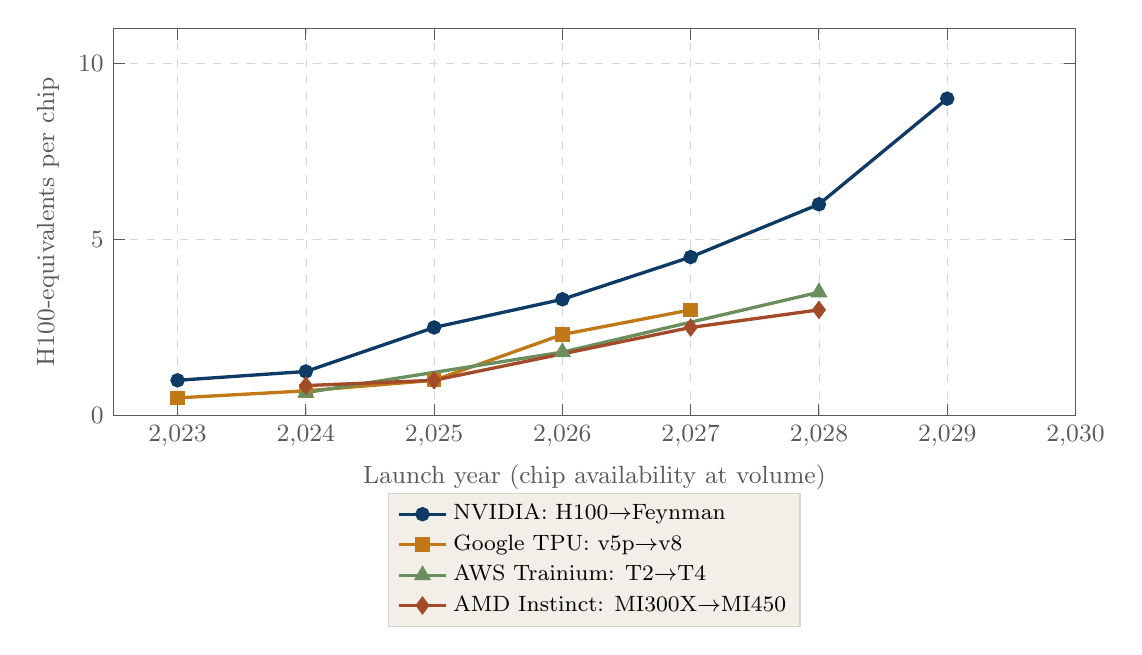
\begin{tikzpicture}
\begin{axis}[
  width=13.8cm, height=6.5cm,
  xlabel={Launch year (chip availability at volume)},
  ylabel={H100-equivalents per chip},
  xlabel style={font=\small,color=softGrey},
  ylabel style={font=\small,color=softGrey},
  xmin=2022.5, xmax=2030,
  ymin=0, ymax=11,
  xtick={2023,2024,2025,2026,2027,2028,2029,2030},
  xticklabel style={font=\small,color=softGrey},
  yticklabel style={font=\small,color=softGrey},
  axis line style={softGrey,thin},
  tick style={softGrey,thin},
  grid=major, grid style={paleGrey,dashed,very thin},
  legend style={at={(0.5,-0.20)},anchor=north,font=\footnotesize,draw=paleGrey,fill=lightCream,legend columns=1},
  legend cell align={left},
]
% NVIDIA curve
\addplot[color=chartA,line width=1.2pt,mark=*,mark size=2pt] coordinates {
  (2023, 1.0) (2024, 1.25) (2025, 2.5) (2026, 3.3) (2027, 4.5) (2028, 6.0) (2029, 9.0)
};
\addlegendentry{NVIDIA: H100$\rightarrow$Feynman}
% Google TPU curve
\addplot[color=chartB,line width=1.2pt,mark=square*,mark size=2pt] coordinates {
  (2023, 0.5) (2024, 0.7) (2025, 1.0) (2026, 2.3) (2027, 3.0)
};
\addlegendentry{Google TPU: v5p$\rightarrow$v8}
% AWS Trainium curve
\addplot[color=chartC,line width=1.2pt,mark=triangle*,mark size=2.4pt] coordinates {
  (2024, 0.65) (2026, 1.8) (2028, 3.5)
};
\addlegendentry{AWS Trainium: T2$\rightarrow$T4}
% AMD Instinct curve
\addplot[color=chartD,line width=1.2pt,mark=diamond*,mark size=2.4pt] coordinates {
  (2024, 0.85) (2025, 1.0) (2027, 2.5) (2028, 3.0)
};
\addlegendentry{AMD Instinct: MI300X$\rightarrow$MI450}
\end{axis}
\end{tikzpicture}
\caption{Per-chip H100-equivalents by chip family and launch year. NVIDIA holds per-chip leadership, but AWS Trainium~3 and Google TPU~v7 Ironwood close the gap in 2026--2027. 2028--2029 figures (Feynman, Trainium~4, TPU~v9, MI450) are roadmap-projected and subject to tape-out and yield.\protect\footnotemark}
\end{figure}
\footnotetext{Per-chip H100e values computed from published 8-bit OP/s throughput disclosures: NVIDIA GTC keynotes 2023--2026; Google Cloud Next 2025--2026 TPU specifications; AWS re:Invent 2023--2025 Trainium disclosures; AMD Advancing AI events 2023--2025. Post-2027 values extrapolated from roadmap announcements and are explicitly projections, not confirmed silicon.}

\subsection{Chip vendor share across the Western horizon}

Aggregating the chip commitments across the hyperscaler, frontier-lab, and neocloud segments for the full 2030 horizon produces a vendor-share distribution that differs markedly from the 2024--2025 marketplace.

\begin{figure}[htbp]
\centering
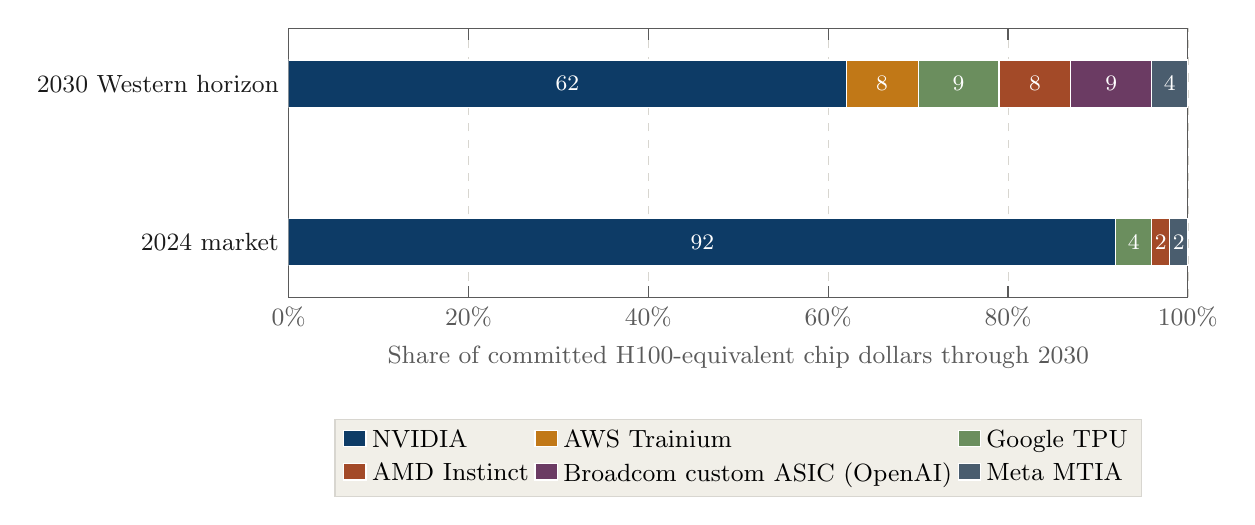
\begin{tikzpicture}
\begin{axis}[
  width=13.0cm, height=5cm,
  xbar stacked,
  bar width=0.6cm,
  enlarge y limits=0.35,
  symbolic y coords={y2024,y2030},
  ytick=data,
  yticklabels={2024 market,2030 Western horizon},
  xlabel={Share of committed H100-equivalent chip dollars through 2030},
  xlabel style={font=\small,color=softGrey},
  yticklabel style={font=\small,color=inkBlack},
  xticklabel style={font=\small,color=softGrey},
  xmin=0, xmax=100,
  xtick={0,20,40,60,80,100},
  xticklabel={\pgfmathprintnumber{\tick}\%},
  axis line style={softGrey,thin},
  tick style={softGrey,thin},
  grid=major, grid style={paleGrey,dashed,very thin},
  legend style={at={(0.5,-0.45)},anchor=north,font=\small,draw=paleGrey,fill=lightCream,legend columns=3},
  legend cell align={left},
  nodes near coords,
  nodes near coords style={font=\footnotesize,color=white,align=center},
  every node near coord/.append style={/pgf/number format/.cd,fixed,precision=0},
]
\addplot[fill=chartA,draw=white] coordinates {(92,y2024) (62,y2030)};
\addlegendentry{NVIDIA}
\addplot[fill=chartB,draw=white] coordinates {(0,y2024) (8,y2030)};
\addlegendentry{AWS Trainium}
\addplot[fill=chartC,draw=white] coordinates {(4,y2024) (9,y2030)};
\addlegendentry{Google TPU}
\addplot[fill=chartD,draw=white] coordinates {(2,y2024) (8,y2030)};
\addlegendentry{AMD Instinct}
\addplot[fill=chartE,draw=white] coordinates {(0,y2024) (9,y2030)};
\addlegendentry{Broadcom custom ASIC (OpenAI)}
\addplot[fill=chartF,draw=white] coordinates {(2,y2024) (4,y2030)};
\addlegendentry{Meta MTIA}
\end{axis}
\end{tikzpicture}
\caption{Share of committed chip-capital dollars by vendor, 2024 vs.\ 2030 Western horizon. NVIDIA holds majority share but cedes roughly 30 percentage points to AWS, Google, AMD, Broadcom, and Meta combined.\protect\footnotemark}
\end{figure}
\footnotetext{Author's aggregation from operator-disclosed chip commitments: Anthropic Project Rainier (Trainium); Anthropic TPU (1M chips + 3.5 GW expansion); OpenAI--NVIDIA (10 GW), OpenAI--AMD (6 GW Instinct), OpenAI--Broadcom (10 GW custom ASIC); Meta MTIA deployment commentary; Microsoft--NVIDIA Fairwater silicon. Individual percentage estimates carry material uncertainty because most commitments are disclosed in GW or chip-count rather than dollar terms; dollar share derived using vendor-specific ASP assumptions.}

\subsection{The commercial reality of Anthropic's silicon}

Anthropic's disclosed silicon posture is worth pausing on because it illustrates the commercial distance between ``NVIDIA-dominant'' as a marketplace observation and ``NVIDIA-exclusive'' as a training decision for a specific lab. Anthropic's largest training cluster today is the Amazon-operated New Carlisle campus, which runs \textbf{AWS Trainium~2} as its primary accelerator.\footnote{Anthropic and Amazon, \emph{Anthropic and Amazon expand collaboration for up to 5 gigawatts of new compute}, April 20, 2026, \url{https://www.anthropic.com/news/anthropic-amazon-compute}.} Anthropic's second-largest committed training capacity is the Google-operated TPU programme, at \textbf{up to one million TPU chips plus 3.5 GW of TPU v7/v8 capacity from 2027 onward}. Anthropic's NVIDIA deployment, via Nscale-Fluidstack and Microsoft-Azure, is material but secondary to both Trainium and TPU on a dollar-weighted basis.

Put differently: the single largest non-NVIDIA training buildout at the global frontier today is happening at Anthropic, on AWS silicon. The ``NVIDIA has won AI'' framing understates how far chip-diversification has already travelled at the lab tier.

\subsection{H100e sensitivity: conservative, base, aggressive silicon uplift}
\label{subsec:h100e-sensitivity}

The paper's headline figure of 78.0M H100-equivalents by 2030 assumes per-family chip-density trajectories drawn from disclosed roadmaps through 2027 and extrapolations of observed per-generation uplift curves for 2028--2030. The rounded 78.0M manuscript convention is distinct from the separate 78.2M chip-layer estimate used in sensitivity notes. That extrapolation is load-bearing: small shifts in the 2028--2030 density assumption move the aggregate H100e count by tens of millions.

What H100-equivalents miss. Before presenting the sensitivity range, three caveats: (i) H100e normalizes 8-bit dense FLOP/s but understates gains in sparsity, lower-precision (FP4/FP6) inference, and memory-bandwidth throughput that matter disproportionately for reasoning-dominated workloads; (ii) networking fabric (NVLink/NVSwitch generations, InfiniBand NDR/XDR, AWS EFAv3) contributes 10--30\% of effective-throughput differences between nominally-equivalent chips; (iii) compiler maturity (CUDA vs XLA vs Neuron) and cluster utilization (discussed in \S9) further decouple nameplate H100e from delivered training throughput. Readers should treat H100e as the least-bad available scalar, not a physical-FLOP count.

\begin{table}[htbp]
\centering
\small
\begin{tabular}{@{}lrr@{}}
\toprule
\textbf{Scenario} & \textbf{2030 Western H100e (M)} & \textbf{Growth vs.\ 2026 Q2} \\
\midrule
Conservative (hold 2026 density flat) & 60.0 & 14.3$\times$ \\
Base (disclosed roadmaps + observed curves) & 78.0 & 18.6$\times$ \\
Aggressive (straight-line Epoch per-family curve) & 110.0 & 26.2$\times$ \\
\bottomrule
\end{tabular}
\caption{H100-equivalent count in the 2030 Western horizon under three silicon-uplift scenarios. Conservative holds per-family density flat at 2026 levels; aggressive extrapolates Epoch's observed per-family curve (~2$\times$ NVIDIA, ~1.7$\times$ TPU, ~2.2$\times$ Trainium per generation, 2022--2026).}
\end{table}

Per-family disclosure status underlying the base case: NVIDIA H100/H200/B200/B300 are disclosed via GTC keynotes and datasheet material; Rubin is roadmap-only through 2027 and extrapolated 2028--2030. Google TPU v5p/v5e/v6/v7~Ironwood/v8 are disclosed through 2026; TPU v9 is inferred. AWS Trainium~2 is disclosed; Trainium~3 is roadmap-disclosed at re:Invent 2025; Trainium~4 is extrapolated. AMD MI300X/MI325X are disclosed; MI400 is roadmap-disclosed; MI450 is inferred. Broadcom custom ASIC (Anthropic XPU, OpenAI XPU, Meta MTIA): disclosed at GW-commitment level, not chip-count or per-chip-throughput level; the silicon-layer contribution from Broadcom programs is the single largest source of aggressive-case upside (and the largest unknown).

The $\pm$30\% uncertainty band around the 78.0M H100e base reading is not precision-inflation: it reflects honest extrapolation risk across six chip families, three foundries (TSMC, Samsung, Intel-foundry), and five compressed cycles of 2-year generational cadence. Anyone forecasting a single H100e number for 2030 without a sensitivity band is overconfident.

% ============================================================================
\section{The \$2 trillion question: where the money comes from}
\label{sec:capital}
% ============================================================================

The 47.9~GW facility Western horizon (40.9~GW IT-load bridge) carries an estimated \textbf{capital envelope of approximately \$1.77~trillion between 2026 and 2030} (range \$1.44--2.25~T across operator mix and BTM-generation share; per-layer derivation in \texttt{anatomy\_layer\_costs.yaml}). A separate approximately \textbf{\$550~billion of contracted remaining performance obligations (RPO)} underwrites but does not constitute this capex --- see \S\ref{subsec:financing-bridge}. The build-out therefore has three distinct financial ledgers: capex requirements, financing sources, and revenue-underwriting commitments.

\subsection{Bucket 1: hyperscaler operating cash flow (actual spend and guided)}

``Who pays'' has four distinct answers in the AI build-out: capex already spent or guided, capex still required, contracted RPO that underwrites future capex, and the financing source that funds it. The Oracle--OpenAI \$300B commitment is contracted revenue for Oracle, Microsoft's \$88B FY25 capex is actual capital expenditure, and Applied Digital's \$2.15B senior secured notes are a financing instrument. These are not substitutes and must not be summed.

The four large US hyperscalers (Microsoft, Amazon, Google, Meta) collectively guided capital expenditures of approximately \textbf{\$400 billion in calendar 2025} and approximately \textbf{\$500 billion in calendar 2026}, with the AI-data-centre share rising from roughly 60\% to 75\% of total capex across the two years.\footnote{Microsoft: FY2025 capex \$88.2B (10-K filed July 31, 2025), FY2026 guided ``meaningfully above'' (Q2 FY2026 earnings, January 28, 2026). Amazon: Andy Jassy Q4 2025 commentary, February 5, 2026: ``We expect 2026 capital expenditures to be notably higher than 2025's \$125B''; \url{https://ir.aboutamazon.com/}. Alphabet: Ruth Porat Q4 2025 commentary, February 4, 2026: ``2026 capital expenditures will be approximately \$85 billion''. Meta: Susan Li Q4 2025 commentary, January 28, 2026: ``2026 total expenses of \$175--\$200B ... capital expenditures of \$80--\$95B''. Sources: respective Q4 2025 earnings calls and subsequent 10-K filings.} Across two years, the four-hyperscaler aggregate is roughly \textbf{\$550--650 billion of AI-attributable capex}, which alone funds more than a third of the 2030 horizon.

\begin{figure}[htbp]
\centering
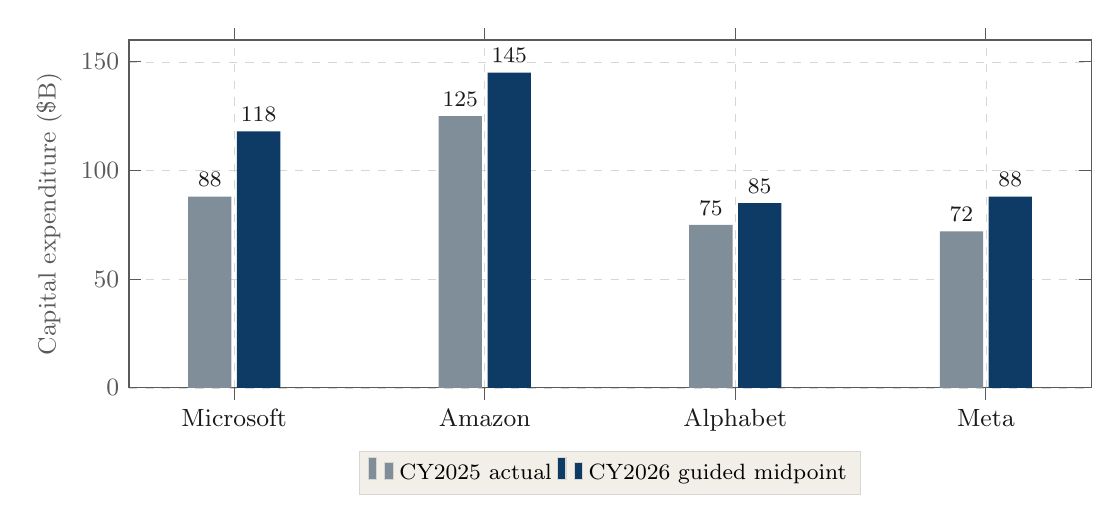
\begin{tikzpicture}
\begin{axis}[
  width=13.8cm, height=6cm,
  ybar,
  bar width=0.55cm,
  enlarge x limits=0.14,
  symbolic x coords={Microsoft, Amazon, Alphabet, Meta},
  xtick=data,
  xticklabel style={font=\small,color=inkBlack},
  ylabel={Capital expenditure (\$B)},
  ylabel style={font=\small,color=softGrey},
  yticklabel style={font=\small,color=softGrey},
  ymin=0, ymax=160,
  axis line style={softGrey,thin},
  tick style={softGrey,thin},
  grid=major, grid style={paleGrey,dashed,very thin},
  legend style={at={(0.5,-0.18)},anchor=north,font=\footnotesize,draw=paleGrey,fill=lightCream,legend columns=2},
  legend cell align={left},
  nodes near coords,
  nodes near coords style={font=\footnotesize,color=inkBlack,anchor=south},
]
\addplot[fill=chartF!70,draw=none] coordinates {(Microsoft, 88) (Amazon, 125) (Alphabet, 75) (Meta, 72)};
\addlegendentry{CY2025 actual}
\addplot[fill=chartA,draw=none] coordinates {(Microsoft, 118) (Amazon, 145) (Alphabet, 85) (Meta, 88)};
\addlegendentry{CY2026 guided midpoint}
\end{axis}
\end{tikzpicture}
\caption{Big-Four hyperscaler capex, CY2025 actual and CY2026 guidance midpoints. The AI-data-center share has risen from roughly 60\% in CY2024 to 75\% in CY2026 guidance.\protect\footnotemark}
\end{figure}
\footnotetext{CY2025 actuals: Microsoft FY2025 10-K; Amazon Q4 2025 earnings (FY = CY); Alphabet Q4 2025 earnings (FY = CY); Meta Q4 2025 earnings (FY = CY). CY2026 guidance: from respective Q4 2025 earnings calls and subsequent 10-K filings as of April 2026. Microsoft FY2026 figures adjusted to a calendar-year basis by linear interpolation across the June-ending fiscal year.}

\subsection{Bucket 2: contracted RPO (revenue obligations, not capex)}
\label{subsec:rpo-bucket}

The single largest contracted-revenue commitment in the history of enterprise cloud is the Oracle--OpenAI agreement, disclosed in Oracle's Q1 FY2026 10-Q as a \textbf{\$300 billion five-year take-or-pay commitment from OpenAI} beginning in 2027.\footnote{Oracle Corporation, Form 10-Q for Q1 FY2026, filed September 10, 2025. Oracle disclosed ``a \$300 billion, five-year purchase commitment'' from a named customer (subsequently confirmed as OpenAI in Oracle's Q2 FY2026 earnings call, December 9, 2025, Larry Ellison). \url{https://www.sec.gov/cgi-bin/browse-edgar}} The Oracle--OpenAI commitment is the single largest capex-underwriting contract signed in the industry. \textbf{It is a revenue obligation from OpenAI to Oracle, not a capex channel:} the \$300~B appears in Oracle's income statement as contracted future revenue, and separately enables Oracle to finance Stargate shell construction via a combination of corporate debt, SPV debt, and retained earnings. In this paper it is counted in the RPO bucket (\S\ref{subsec:financing-bridge}), not in the capex bucket.

Additional take-or-pay commitments include: \textbf{Anthropic--Amazon at ``more than \$100 billion over ten years''} (April 20, 2026 announcement);\footnote{Anthropic and Amazon, April 20, 2026. Amazon's 10-K will disclose aggregate RPO from this agreement in Q2 FY2026 filings.} \textbf{Anthropic--Google TPU estimated at \$52--60 billion} based on the ``up to one million chips'' language and published TPU v7 pricing;\footnote{Anthropic, \emph{Expanding our use of Google Cloud TPUs and Services}, October 23, 2025, and Google Cloud Press Corner, \emph{Anthropic to Expand Use of Google Cloud TPUs and Services}, October 23, 2025, support up to one million TPUs, well over a GW coming online in 2026, and tens of billions of dollars. Google's April 6, 2026 press release supports multiple GW of TPU capacity starting in 2027. The \$52--60B value is an industry estimate, not an Alphabet filing.} \textbf{CoreWeave--Microsoft and CoreWeave--OpenAI at a combined approximately \$50 billion in 15-year take-or-pay}, already reflected in CoreWeave's \$60.7 billion FY2025 RPO.\footnote{CoreWeave, Inc.\ FY2025 10-K, Note~12 (Contract Balances), disclosing RPO of \$60.7~billion. Microsoft contract announced 2022; OpenAI contract announced March 2025.} \textbf{Nebius--Meta at up to approximately \$27 billion} (March 16, 2026);\footnote{Nebius, \emph{Nebius signs new AI infrastructure agreement with Meta}, March 16, 2026, \url{https://nebius.com/newsroom/nebius-signs-new-ai-infrastructure-agreement-with-meta}.} and \textbf{Nebius--Microsoft at approximately \$19.4 billion}.\footnote{Reuters, September 2025, reporting disclosed Nebius--Microsoft contract value. Nebius aggregate RPO disclosed in Q4 FY2025 shareholder letter; individual counterparty values not separately disclosed by Nebius.}

\subsection{Bucket 3: neocloud debt (financing source, not capex)}

The merchant-neocloud segment has become a significant debt issuer over 2024--2026, supported by the investment-grade counterparty credit behind the take-or-pay revenue. Applied Digital's \textbf{\$2.15 billion of 6.75\% senior secured notes due 2031}, issued March 2026 at an A3 Moody's rating on the SPV pledged to the CoreWeave Ellendale lease, exemplifies the model.\footnote{Applied Digital Corporation, Form 8-K filed March 30, 2026; Moody's Investors Service rating action, March 30, 2026.} CoreWeave has issued multiple tranches of delayed-draw term loans secured by its GPU fleet, collectively in the \$15--20 billion range, against the Microsoft/OpenAI 15-year RPO backlog.\footnote{CoreWeave FY2025 10-K, Note~7 (Debt). Credit agreements with Blackstone, Magnetar, and various other private-credit lenders.}

\subsection{Bucket 4: sovereign wealth (financing source)}

Abu Dhabi's MGX, Saudi Arabia's Public Investment Fund (through HUMAIN), Reliance Industries (India), and the UK government's Department for Science, Innovation and Technology (DSIT) together contribute an estimated \textbf{\$150--250 billion of state-backed capital} to the global AI buildout 2026--2030.\footnote{MGX is a 2025-formed Abu Dhabi sovereign AI investment vehicle, partnered in the OpenAI Stargate consortium (\$100~B initial tranche, \$500~B ten-year vehicle per January 21, 2025 OpenAI release). HUMAIN is the Saudi Public Investment Fund's AI subsidiary (incorporated March 2025), deploying the \$10 billion AMD joint venture and the xAI sovereign 500~MW campus. UK DSIT's AI Opportunities Action Plan commits approximately £5 billion (announced January 13, 2025, \url{https://www.gov.uk/government/publications/ai-opportunities-action-plan}). Reliance Industries: Mukesh Ambani's 47th AGM address, August 29, 2024, references ``gigawatt-scale'' capacity at Jamnagar.} Because sovereign-AI programmes carry structurally different revenue models and grid-connection dynamics, they are described separately in Section~8.

\subsection{Capex bridge: what the money pays for}
\label{subsec:capex-bridge}

The \$1.77~trillion capital envelope decomposes across five distinct capex categories derived from the bottoms-up unit-economics decomposition in \texttt{anatomy\_layer\_costs.yaml} (cross-referenced to Crusoe Abilene, Meta Hyperion, Bernstein, Epoch, McKinsey, and JLL anchors). Understanding the split matters because the supply-chain, permitting, and execution risk differs sharply across them: physical shells have a 24--36 month lead time, accelerators are constrained by wafer-start and HBM capacity, power and cooling infrastructure hinges on utility and substation delivery, networking scales more linearly with demand, and land/permitting is one-time.

\begin{table}[htbp]
\centering
\small
\begin{tabularx}{\textwidth}{@{}>{\raggedright\arraybackslash}Xrr>{\raggedright\arraybackslash}X@{}}
\toprule
\textbf{Capex category} & \textbf{\$B (low)} & \textbf{\$B (high)} & \textbf{Binding constraint} \\
\midrule
Accelerator + server BOM (rack-complete) & 830 & 1{,}195 & TSMC CoWoS + HBM \\
Shell + civil + land + base/AI fit-out & 230 & 505 & 24--36 mo build cycle \\
Cooling stack & 105 & 180 & DLC supply chain (Vertiv, Schneider, Motivair, AWS IRHX) \\
Power infrastructure (substation, transformer, switchgear, UPS, BTM gen) & 100 & 285 & 80--128 wk LPT lead; gas turbines sold out 2028+ \\
Out-of-rack networking + storage & 145 & 275 & Broadcom T5/T6, NVIDIA Spectrum-X, optics \\
Grid interface + assigned upgrades & 15 & 260 & ISO/RTO queue, customer-funded transmission \\
\midrule
\textbf{Total capital envelope} & \textbf{1{,}399} & \textbf{2{,}192} & central \textbf{\$1{,}726} \\
\bottomrule
\end{tabularx}
\caption{Western 2026--2030 capital envelope by capex category. Accelerator and server BOM is the dominant share (~53\% of central) because per-chip ASPs in the B300/Rubin/Trainium-3 era are \$30--50k+ at densities of 415--440 chips per facility-MW. Defensible range \$1.44--2.25~T; per-component build-up in \texttt{anatomy\_layer\_costs.yaml}.}
\end{table}

\subsection{Financing bridge: sources of funds}
\label{subsec:financing-bridge}

The same capital envelope can be equivalently decomposed by source-of-funds. The capex bridge and the financing bridge are distinct accounting questions: the first asks what the money pays for, the second asks whose balance sheet it flows off. They reconcile at the central but use different convention bounds (arithmetic-extreme for capex, credible-source for financing); see the capex bridge and financing bridge captions below for the respective range derivations.

\begin{table}[htbp]
\centering
\small
\begin{tabular}{@{}lrrl@{}}
\toprule
\textbf{Financing source} & \textbf{\$B (low)} & \textbf{\$B (high)} & \textbf{Balance-sheet impact} \\
\midrule
Hyperscaler operating cash flow & 800 & 950 & Retained earnings \\
Corporate debt (hyperscaler \& neocloud) & 250 & 380 & Corporate credit \\
SPV / project-finance debt & 250 & 380 & Off-balance-sheet; IG-wrapped \\
Sovereign wealth (MGX, PIF, DSIT, RIL) & 200 & 320 & State balance sheet \\
Equity (public markets + private) & 150 & 220 & Founder dilution; VC LPs \\
\midrule
\textbf{Total capital envelope} & \textbf{1{,}400} & \textbf{2{,}190} & central \textbf{\$1{,}730} \\
\bottomrule
\end{tabular}
\caption{Financing-source decomposition of the \$1.77~T capital envelope. Hyperscaler operating cash flow dominates: Microsoft, Amazon, Google, and Meta collectively generate roughly \$400~B of pre-capex free cash flow annually, with 2026 capex guidance of approximately \$500~B (75\% AI-attributable). SPV / project-finance debt is structured against 15-year take-or-pay RPO and wrapped to investment-grade. Sovereign and equity sit separately.}
\end{table}

The important conceptual separation: the \textbf{\$550B of contracted RPO} (Oracle--OpenAI \$300B, Anthropic--Amazon \$100B+, Anthropic--Google \$52--60B, Nebius--Meta \$27B, Nebius--Microsoft \$19.4B, CoreWeave--Microsoft/OpenAI \$50B) is \emph{not} a capex source. It is a \emph{revenue commitment} from the lab to the infrastructure provider that \emph{underwrites} the infrastructure provider's capex. Oracle's \$300B OpenAI commitment appears in Oracle's income statement as future revenue, not in Oracle's capex line. That same \$300B enables Oracle to finance Stargate shell construction through some combination of corporate debt, SPV debt, and retained earnings, which is why RPO shows up as the right-hand column of the financing bridge interpretation, not as a free-standing sixth bucket.

\subsection{The aggregate: capex bridge and financing bridge}

The \$1.77~T capital envelope has two equally valid aggregate views. The capex bridge below shows \emph{what the money physically buys}; the financing bridge shows \emph{whose balance sheet the money flows off}. The two views reconcile at the \$1.77~T central but use different convention bounds (arithmetic layer-extreme for the capex bridge \$1.44--2.25~T, credible-source range for the financing bridge); the \$550B of contracted remaining performance obligations (RPO) is \emph{neither} --- it is the revenue underwriting that \emph{enables} the debt-financing channel (Oracle's \$300B from OpenAI, Anthropic's \$100B+ from Amazon, Nebius's \$27B from Meta, etc.\ are lab \emph{revenue} commitments, not capex channels; rev-2 mis-depicted RPO as a stand-alone funding source and is corrected here).

\begin{figure}[htbp]
\centering
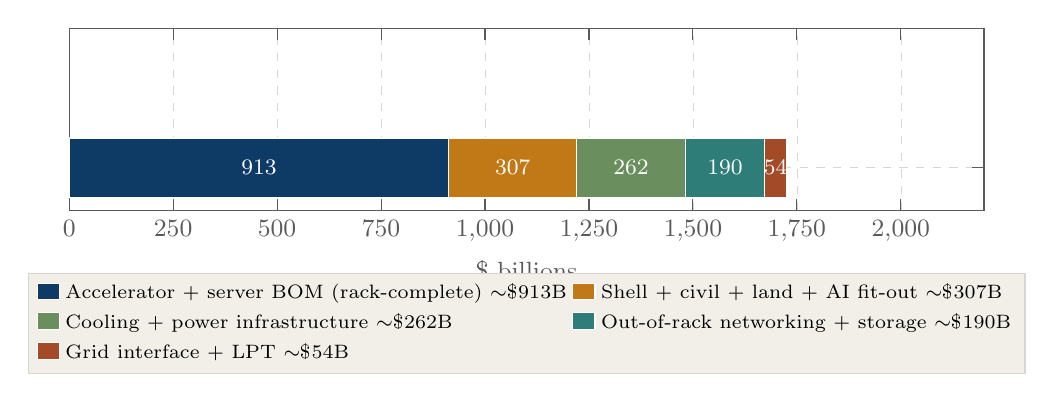
\begin{tikzpicture}
\begin{axis}[
  width=13.2cm, height=3.9cm,
  xbar stacked,
  bar width=0.75cm,
  enlarge y limits=0.45,
  symbolic y coords={capex,dummy},
  ytick={capex},
  yticklabels={},
  xlabel={\$ billions},
  xlabel style={font=\small,color=softGrey},
  yticklabel style={font=\small,color=inkBlack},
  xticklabel style={font=\small,color=softGrey},
  xmin=0, xmax=2200,
  xtick={0,250,500,750,1000,1250,1500,1750,2000},
  axis line style={softGrey,thin},
  tick style={softGrey,thin},
  grid=major, grid style={paleGrey,dashed,very thin},
  legend style={at={(0.5,-0.34)},anchor=north,font=\scriptsize,draw=paleGrey,fill=lightCream,legend columns=2},
  legend cell align={left},
  nodes near coords,
  nodes near coords style={font=\footnotesize,color=white,align=center},
  every node near coord/.append style={/pgf/number format/.cd,fixed,precision=0},
]
\addplot[fill=chartA,draw=white] coordinates {(913,capex)};
\addlegendentry{Accelerator + server BOM (rack-complete) $\sim$\$913B}
\addplot[fill=chartB,draw=white] coordinates {(307,capex)};
\addlegendentry{Shell + civil + land + AI fit-out $\sim$\$307B}
\addplot[fill=chartC,draw=white] coordinates {(262,capex)};
\addlegendentry{Cooling + power infrastructure $\sim$\$262B}
\addplot[fill=chartG,draw=white] coordinates {(190,capex)};
\addlegendentry{Out-of-rack networking + storage $\sim$\$190B}
\addplot[fill=chartD,draw=white] coordinates {(54,capex)};
\addlegendentry{Grid interface + LPT $\sim$\$54B}
\addplot[draw=none,fill=none,forget plot,nodes near coords={}] coordinates {(0,dummy)};
\end{axis}
\end{tikzpicture}
\caption{Capex bridge for the \$1.77~T envelope (range \$1.44--2.25~T). Accelerator and server BOM (silicon plus in-rack mechanical) is approximately 53\%; shell, civil, land, and AI fit-out approximately 18\%; cooling and power infrastructure approximately 15\% combined; out-of-rack networking and storage approximately 11\% (3--6$\times$ more networking-heavy per MW than legacy cloud); grid interface and transformers the remaining 3\%.\protect\footnotemark}
\end{figure}
\footnotetext{Bottoms-up aggregation: per-layer \$/MW central case from \texttt{anatomy\_layer\_costs.yaml} multiplied by 47.9~GW raw announced facility horizon. Accelerator + server BOM: 440 GB200-class chips per facility-MW at \$45k all-in chip-plus-rack-share (\$19.5M/MW central rack-complete). Cross-anchored to Bernstein per-rack BOM (\$3.9M loaded NVL72), Crusoe Abilene disclosed shell-only \$12.5M/MW, and the cross-forecaster reconciliation in \texttt{forecaster\_capex\_comparison.yaml}.}

\textbf{The \$550B RPO is revenue underwriting, not a funding channel.} Between the capex bridge and the financing bridge lies the \$550B in contracted remaining performance obligations disclosed in the hyperscaler and neocloud 10-K filings. Oracle's \$300B from OpenAI, Anthropic's \$100B+ from Amazon, Anthropic's \$52--60B from Google, Nebius's \$27B from Meta, Nebius's \$19.4B from Microsoft, and CoreWeave's approximately \$50B from Microsoft and OpenAI together constitute \emph{revenue} commitments from labs to infrastructure providers. That revenue backing is what enables the infrastructure provider's SPV or corporate debt to be wrapped to investment grade; it is the credit-enhancement spine of the debt channel, not a stand-alone funding bucket.

\begin{figure}[htbp]
\centering
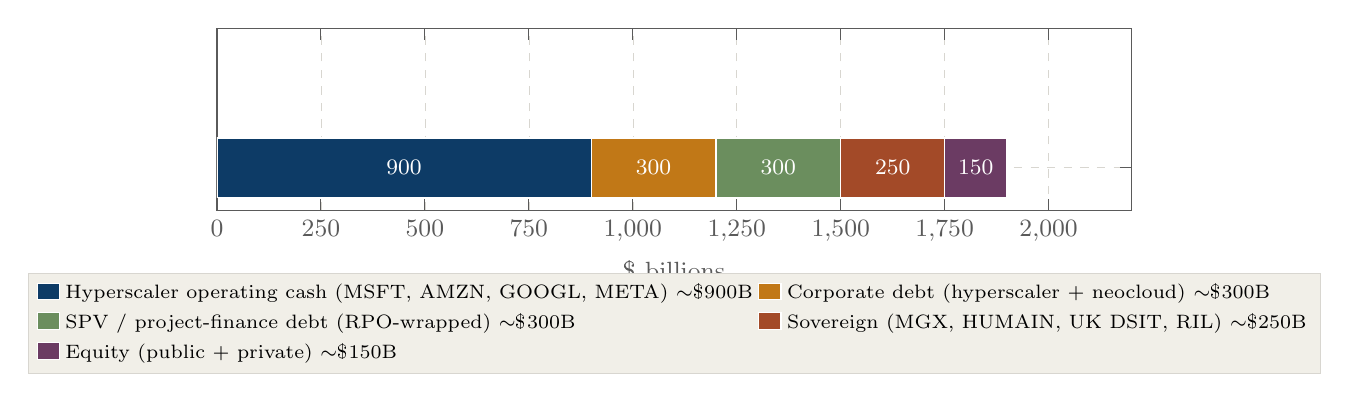
\begin{tikzpicture}
\begin{axis}[
  width=13.2cm, height=3.9cm,
  xbar stacked,
  bar width=0.75cm,
  enlarge y limits=0.45,
  symbolic y coords={financing,dummy},
  ytick={financing},
  yticklabels={},
  xlabel={\$ billions},
  xlabel style={font=\small,color=softGrey},
  yticklabel style={font=\small,color=inkBlack},
  xticklabel style={font=\small,color=softGrey},
  xmin=0, xmax=2200,
  xtick={0,250,500,750,1000,1250,1500,1750,2000},
  axis line style={softGrey,thin},
  tick style={softGrey,thin},
  grid=major, grid style={paleGrey,dashed,very thin},
  legend style={at={(0.5,-0.34)},anchor=north,font=\scriptsize,draw=paleGrey,fill=lightCream,legend columns=2},
  legend cell align={left},
  nodes near coords,
  nodes near coords style={font=\footnotesize,color=white,align=center},
  every node near coord/.append style={/pgf/number format/.cd,fixed,precision=0},
]
\addplot[fill=chartA,draw=white] coordinates {(900,financing)};
\addlegendentry{Hyperscaler operating cash (MSFT, AMZN, GOOGL, META) $\sim$\$900B}
\addplot[fill=chartB,draw=white] coordinates {(300,financing)};
\addlegendentry{Corporate debt (hyperscaler + neocloud) $\sim$\$300B}
\addplot[fill=chartC,draw=white] coordinates {(300,financing)};
\addlegendentry{SPV / project-finance debt (RPO-wrapped) $\sim$\$300B}
\addplot[fill=chartD,draw=white] coordinates {(250,financing)};
\addlegendentry{Sovereign (MGX, HUMAIN, UK DSIT, RIL) $\sim$\$250B}
\addplot[fill=chartE,draw=white] coordinates {(150,financing)};
\addlegendentry{Equity (public + private) $\sim$\$150B}
\addplot[draw=none,fill=none,forget plot,nodes near coords={}] coordinates {(0,dummy)};
\end{axis}
\end{tikzpicture}
\caption{Financing bridge for the \$1.77~T envelope by source of funds. Hyperscaler operating cash flow dominates; corporate and SPV debt are the second channel (SPV wrapped to investment-grade against 15-year take-or-pay RPO); sovereign and equity sit separately. The \$550~B of RPO does not appear here as a standalone source --- it is the revenue underwriting that enables the SPV debt channel.\protect\footnotemark}
\end{figure}
\footnotetext{Author's aggregation. Hyperscaler channel: Big-Four CY2025 actual (~\$400~B) + CY2026 guidance (~\$500~B) times 75\% AI share, extended 2027--2030 at roughly flat dollar levels per current capex-cycle commentary. Corporate debt: hyperscaler balance-sheet additions plus CoreWeave, Nebius, Applied Digital, Crusoe corporate issuance. SPV / project-finance: Applied Digital--CoreWeave SPV (\$2.15~B 6.75\% senior secured 2031, A3), CoreWeave Blackstone facility, Nebius ABS, Crusoe \$9.6~B JPMorgan-led debt + Blue Owl JV --- all wrapped to investment-grade via lab-revenue RPO. Sovereign: MGX \$100--200B per OpenAI Stargate announcement + HUMAIN \$10B AMD JV + UK DSIT £5B + RIL estimated \$30--50B Jamnagar phase-one. Equity: OpenAI secondary rounds, Anthropic Series F/G, CoreWeave public-float, Nebius AMS float, Crusoe Series E (\$1.375B at \textgreater\$10B valuation, October 2025).}

% ============================================================================
\section{What prevents a gigawatt from becoming operational?}
\label{sec:execution-risk}
% ============================================================================

The principal execution risks fall into four categories: grid interconnection, chip delivery, counterparty concentration, and the realization of outer-year stretch targets (Meta Hyperion, Reliance Jamnagar, and the Anthropic--Amazon full 5~GW in particular). Each is priced into the scenario matrix in \S\ref{subsec:stress-matrix}.

\subsection{Confidence decomposition of the 2030 horizon}

The 47.9~GW announced horizon splits across the six evidence tiers as 6.52~GW T1 Operational (100\% realization probability), 11.91~GW T2 Under construction (88\%), 4.50~GW T3 Firm commercial (78\%), 15.79~GW T4 Announced site plan (58\%), 8.86~GW T5 LOI or stretch target (32\%), and 0.33~GW T6 Analyst inference (25\%). Probability weighting yields a \textbf{32.6~GW central case}, between the 22.9~GW firm-evidence-only reading and the 47.9~GW announced ceiling.

\begin{figure}[htbp]
\centering
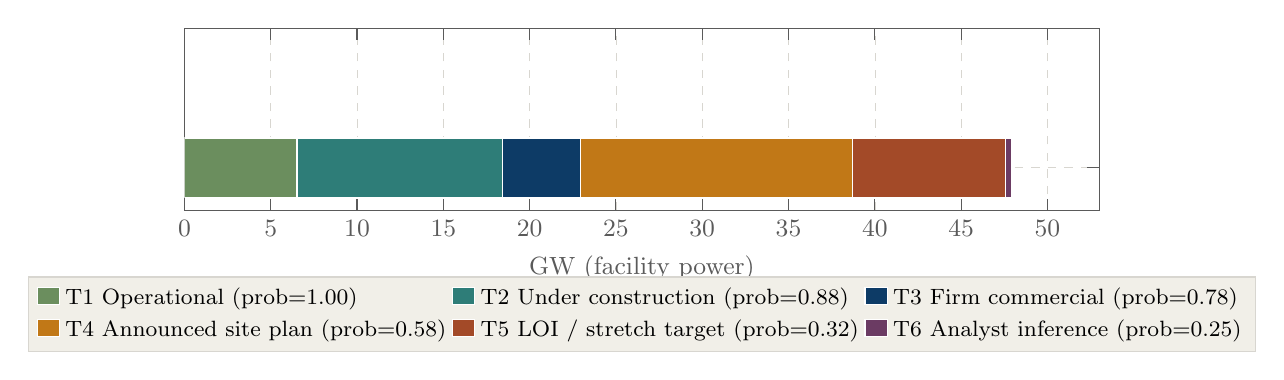
\begin{tikzpicture}
\begin{axis}[
  width=13.2cm, height=3.9cm,
  xbar stacked,
  bar width=0.75cm,
  enlarge y limits=0.45,
  symbolic y coords={horizon,dummy},
  ytick={horizon},
  yticklabels={},
  xlabel={GW (facility power)},
  xlabel style={font=\small,color=softGrey},
  yticklabel style={font=\small,color=inkBlack},
  xticklabel style={font=\small,color=softGrey},
  xmin=0, xmax=53,
  axis line style={softGrey,thin},
  tick style={softGrey,thin},
  grid=major, grid style={paleGrey,dashed,very thin},
  legend style={at={(0.5,-0.36)},anchor=north,font=\footnotesize,draw=paleGrey,fill=lightCream,legend columns=3},
  legend cell align={left},
]
\addplot[fill=accentSage,draw=white] coordinates {(6.52,horizon)};
\addlegendentry{T1 Operational (prob=1.00)}
\addplot[fill=chartG,draw=white] coordinates {(11.91,horizon)};
\addlegendentry{T2 Under construction (prob=0.88)}
\addplot[fill=chartA,draw=white] coordinates {(4.50,horizon)};
\addlegendentry{T3 Firm commercial (prob=0.78)}
\addplot[fill=accentOchre,draw=white] coordinates {(15.79,horizon)};
\addlegendentry{T4 Announced site plan (prob=0.58)}
\addplot[fill=accentTerracotta,draw=white] coordinates {(8.86,horizon)};
\addlegendentry{T5 LOI / stretch target (prob=0.32)}
\addplot[fill=chartE,draw=white] coordinates {(0.33,horizon)};
\addlegendentry{T6 Analyst inference (prob=0.25)}
\addplot[draw=none,fill=none,forget plot,nodes near coords={}] coordinates {(0,dummy)};
\end{axis}
\end{tikzpicture}
\caption{The 47.9~GW Western 2030 horizon split across six evidence tiers. Realization probability is the tier-default midpoint with per-row override possible; the probability-weighted sum is \textbf{32.6~GW facility}.\protect\footnotemark}
\end{figure}
\footnotetext{Tier thresholds. \textbf{T1 Operational}: power online in Q2 2026 from Epoch site disclosures and directly disclosed neocloud capacity. \textbf{T2 Under construction}: Epoch sites with active construction visible via satellite or permit and timeline 2026--2027, plus the Microsoft Fairwater International (Norway and UK) build. \textbf{T3 Firm commercial}: 15-year take-or-pay contracts with investment-grade counterparties (CoreWeave--Microsoft, CoreWeave--OpenAI, Nebius--Meta, Applied Digital--CoreWeave). \textbf{T4 Announced site plan}: Epoch sites scheduled 2028 plus overlay commitments with named site, operator, and source-backed plan (notably the Anthropic--AWS incremental, Crusoe Cheyenne, and the smaller neocloud anchors). \textbf{T5 LOI or stretch target}: Epoch sites scheduled 2029--2030, the Meta Hyperion stretch delta, and the Anthropic--Google/Broadcom physical TPU exposure. \textbf{T6 Analyst inference}: Voltage Park / Lightning and the xAI Colossus~2 residual, totalling 0.33~GW facility. Full atom-level audit in \texttt{row\_level\_audit.csv}.}

\begin{figure}[htbp]
\centering
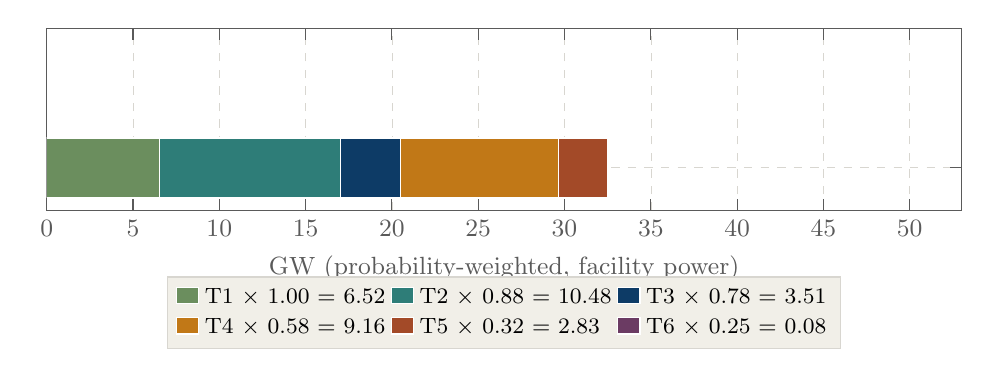
\begin{tikzpicture}
\begin{axis}[
  width=13.2cm, height=3.9cm,
  xbar stacked,
  bar width=0.75cm,
  enlarge y limits=0.45,
  symbolic y coords={horizon,dummy},
  ytick={horizon},
  yticklabels={},
  xlabel={GW (probability-weighted, facility power)},
  xlabel style={font=\small,color=softGrey},
  yticklabel style={font=\small,color=inkBlack},
  xticklabel style={font=\small,color=softGrey},
  xmin=0, xmax=53,
  axis line style={softGrey,thin},
  tick style={softGrey,thin},
  grid=major, grid style={paleGrey,dashed,very thin},
  legend style={at={(0.5,-0.36)},anchor=north,font=\footnotesize,draw=paleGrey,fill=lightCream,legend columns=3},
  legend cell align={left},
]
\addplot[fill=accentSage,draw=white] coordinates {(6.52,horizon)};
\addlegendentry{T1 $\times$ 1.00 = 6.52}
\addplot[fill=chartG,draw=white] coordinates {(10.48,horizon)};
\addlegendentry{T2 $\times$ 0.88 = 10.48}
\addplot[fill=chartA,draw=white] coordinates {(3.51,horizon)};
\addlegendentry{T3 $\times$ 0.78 = 3.51}
\addplot[fill=accentOchre,draw=white] coordinates {(9.16,horizon)};
\addlegendentry{T4 $\times$ 0.58 = 9.16}
\addplot[fill=accentTerracotta,draw=white] coordinates {(2.83,horizon)};
\addlegendentry{T5 $\times$ 0.32 = 2.83}
\addplot[fill=chartE,draw=white] coordinates {(0.08,horizon)};
\addlegendentry{T6 $\times$ 0.25 = 0.08}
\addplot[draw=none,fill=none,forget plot,nodes near coords={}] coordinates {(0,dummy)};
\end{axis}
\end{tikzpicture}
\caption{The same six tiers re-scaled by tier-default realization probability. The probability-weighted 2030 horizon is \textbf{32.6~GW facility}, the right-hand edge of the bar; the T1+T2+T3 firm-evidence subset (22.9~GW announced) is the conservative reading.}
\end{figure}

\subsection{Scenario ranges from 22.9 to 54.2 GW facility}

Four readings of the 2030 horizon sit on a spectrum. The \textbf{firm-evidence-only} case (T1+T2+T3) is approximately \textbf{22.9~GW facility}: operational capacity plus visible construction plus 15-year take-or-pay contracts. Adding the named site plans (T4) brings the \textbf{tier-weighted central case} to approximately \textbf{32.6~GW}. Discarding only the most speculative tier (T5 LOIs and stretch targets) yields a \textbf{raw non-stretch reading} of \textbf{39.0~GW}. The full announced ceiling is \textbf{47.9~GW}, and the row-uncertainty high envelope, in which every stretch lands on its disclosed timeline, is \textbf{54.2~GW}.

\subsection{The grid is the binding constraint in the out-years}

Chip-vendor delivery slippage has historically compressed site-level buildout timelines by three to nine months per generation; NVIDIA Blackwell shipped approximately four months behind its original schedule, and Rubin appears to be tracking to its original late-2026 availability.\footnote{NVIDIA Corporation, Q4 FY2026 earnings, February 26, 2026, Jensen Huang commentary on Rubin shipping commencement: ``Rubin will begin revenue shipments in Q2 calendar 2026, in line with our prior guidance.''} Grid interconnection slippage, by contrast, is structural and approximately \textbf{18 to 30 months on the scheduled interconnect date}, with no comparable compensatory mechanism on the utility side. The combined effect is that \textbf{2028--2029 buildouts carry substantially higher grid-slippage risk than chip-delivery risk}, particularly for the 8--9 GW of the horizon sited in grid-constrained footprints (Northern Virginia residual, the ERCOT West Texas queue, the MISO large-load queue in Wisconsin and Ohio).

\subsection{Scenario architecture: downside, upside, and correlated states}
\label{subsec:stress-matrix}

The 47.9~GW facility announced horizon, 32.6~GW facility deterministic tier-weighted horizon, and 22.9~GW facility conservative horizon are single-path point estimates. The simulation treats them as inputs, not outcomes. It combines tier-level realization uncertainty, named downside shocks, named upside shocks, lab-revenue/RPO stress, and a correlated infrastructure-stress state.

\begin{center}
\footnotesize
\renewcommand{\arraystretch}{1.08}
\setlength{\tabcolsep}{3pt}
\begin{tabular}{@{}L{3.2cm}rrL{6.6cm}r@{}}
\toprule
\textbf{Physical-capacity scenario} & \textbf{$\Delta$GW} & \textbf{$\Delta$\$B capex} & \textbf{Mechanism / counterparties} & \textbf{Prob.} \\
\midrule
Systemic infrastructure stress & $-10.5$ & $-389$ & Correlated grid, financing, and Stargate slippage; replaces Stargate slip, neocloud financing stress, and grid delay in that draw & 15\% \\
Stargate slip & $-3.5$ & $-130$ & Oracle, Microsoft, CoreWeave, SoftBank; conditional probability 17.6\% if systemic stress does not fire & 30\% target \\
Neocloud financing stress & $-2.0$ & $-74$ & CoreWeave, Nebius, Applied Digital, Crusoe; conditional on neither systemic stress nor RPO stress firing, the residual neocloud financing probability is 3.3\%; conditional on RPO stress firing, it is 60\%. Counting systemic stress as including B gives a 25\% total neocloud financing stress target. & 25\% target \\
Grid delay & $-8.0$ & $-296$ & ERCOT, MISO, and PJM delay across xAI, Meta, Stargate, and related large-load sites; conditional probability 29.4\% if systemic stress does not fire & 40\% target \\
Demand/RPO stress & $-2.5$ & $-93$ & Oracle/OpenAI, CoreWeave/Microsoft/OpenAI, Nebius/Meta/Microsoft, Anthropic/AWS/Google; \$100--175B RPO at risk & 15\% \\
Grid/interconnection acceleration & $+2.0$ & $+74$ & Permitting reform, connect-and-manage rules, behind-the-meter generation, and fast-track tariffs & 20\% \\
Neocloud financing upside & $+1.5$ & $+56$ & Tighter SPV and private-credit spreads finance marginal projects earlier & 20\% \\
T4 over-realization & $+2.0$--$2.5$ & $+74$--$93$ & Named-site projects with capex-secured sponsors reach COD faster than tier-default assumptions & 15\% \\
\bottomrule
\end{tabular}
\captionof*{table}{\textbf{Table 5A.} Named scenarios that move the 2030 Western horizon, signed in GW of facility power. Probabilities are subjective; correlation is acknowledged below.}
\end{center}

\begin{center}
\footnotesize
\renewcommand{\arraystretch}{1.08}
\setlength{\tabcolsep}{4pt}
\begin{tabular}{@{}L{3.2cm}rrL{6.6cm}r@{}}
\toprule
\textbf{Silicon / mix scenario} & \textbf{$\Delta$GW} & \textbf{$\Delta$\$B capex} & \textbf{Mechanism} & \textbf{Prob.} \\
\midrule
Chip-roadmap slip & $-1.5$ & $-40$ & NVIDIA, TPU, or Trainium delay by two quarters across the physical-site horizon; H100e impact exceeds facility-GW impact & 50\% \\
Inference mix shift & $0.0$ & $-20$ & Chip-family mix shifts toward inference-optimized silicon; facility-power envelope is unchanged & 55\% \\
Silicon acceleration & $0.0$ & neutral / mildly positive & Rubin, Trainium, TPU, or density-per-watt curve exceeds base case; +8--12M H100e without additional facility power & 25\% \\
\bottomrule
\end{tabular}
\captionof*{table}{\textbf{Table 5B.} Silicon and workload-mix scenarios. These move chip dollars or H100-equivalent capacity rather than utility-meter facility power; silicon acceleration adds compute inside a fixed facility envelope.}
\end{center}

Two features of these scenarios warrant emphasis. First, the largest downside shocks are not independent: a Stargate slip, a neocloud-financing widening, and an ERCOT/MISO interconnection delay tend to fire together in a bad infrastructure-financing state, because all three respond to the same macro variables (rates, equity-market risk appetite, utility-side political pressure). Treating them as independent understates the left tail. We therefore label a systemic-stress state at 15\% probability, in which a combined $-10.5$~GW hit subsumes the three correlated shocks rather than firing them separately; outside that state, the conditional probabilities of the three shocks are calibrated so their unconditional priors stay near 30\%, 25\%, and 40\%.

Second, demand-side stress (Scenario~F) attacks the contracted RPO underwriting that the entire neocloud financing stack rests on. If frontier-lab revenue, API margins, or utilization disappoint, labs may defer, renegotiate, or underutilize their take-or-pay commitments; that subtracts an estimated 2.5~GW from the realized horizon and puts \$100--175~B of contracted revenue at risk. The chip-roadmap slip (Scenario~D) and the inference-mix shift (Scenario~E) are silicon scenarios: the physical GW envelope is largely unchanged, but H100-equivalent capacity and the chip-vendor share of capex move by 10--25\%.

\textbf{Sensitivity to the T4 prior.} T4 is the most judgment-sensitive tier in the rollup: it carries 15.79~GW at a 58\% default realization. Pushing the T4 prior to 45\% lowers the central case to 30.5~GW; pushing it to 70\% raises it to 34.6~GW. The headline central case is therefore stable to within $\pm$2~GW across plausible T4 priors.

% ============================================================================
\section{Sovereign Stretch Annex}
% ============================================================================

Sovereign-backed AI programmes operate under different financing, revenue, and timeline dynamics than the merchant Western build, so they are reported as an annex rather than added to the Western denominator. Six programmes dominate. In the UAE, Stargate UAE (1.40~GW, T4) and Microsoft / G42 Khazna (0.26~GW, T4) are anchor projects under the Abu Dhabi MGX umbrella. In Saudi Arabia, HUMAIN--AMD (500~MW over five years, T4) and HUMAIN--xAI (500~MW JV, Phase 1, T4) are the two PIF-backed programmes; HUMAIN--AMD additionally carries a stated \$10~billion JV envelope. The UK's Culham AI Growth Zone targets 500~MW by 2030 with 100--250~MW by 2027 (T5; no anchor tenant disclosed). India's Reliance pipeline runs across two sites: Jamnagar Phase~1 brings 120~MW online in H2~2026 (T1--T2) under a stated ``gigawatt-scale'' AGM target (T5), and a separate 1.0~GW MoU at Andhra is reported as an additional T5 row. The sovereign aggregate is \textbf{4.96~GW facility announced} (\textbf{3.83~GW} IT-load bridge), \textbf{2.03~GW} probability-weighted. Sovereign upside of 5--7~GW by 2030 is plausible if state-backed programmes scale ahead of disclosure, but it sits outside the Western horizon.

\begin{figure}[htbp]
\centering
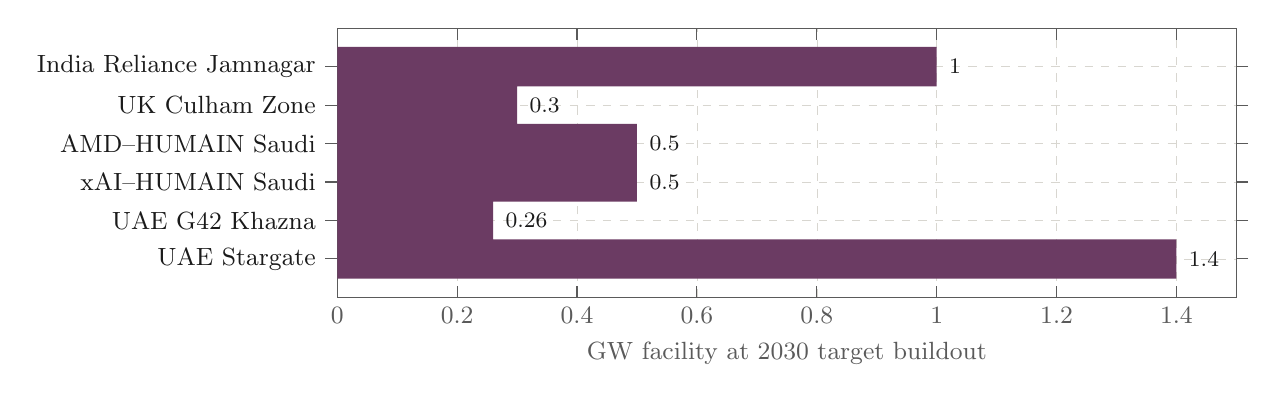
\begin{tikzpicture}
\begin{axis}[
  width=13.0cm, height=5cm,
  xbar,
  bar width=0.5cm,
  enlarge y limits=0.2,
  symbolic y coords={UAE Stargate,UAE Khazna,xAI Saudi,AMD Saudi,UK,India},
  ytick=data,
  yticklabels={UAE Stargate,UAE G42 Khazna,xAI--HUMAIN Saudi,AMD--HUMAIN Saudi,UK Culham Zone,India Reliance Jamnagar},
  xlabel={GW facility at 2030 target buildout},
  xlabel style={font=\small,color=softGrey},
  yticklabel style={font=\small,color=inkBlack},
  xticklabel style={font=\small,color=softGrey},
  xmin=0, xmax=1.5,
  axis line style={softGrey,thin},
  tick style={softGrey,thin},
  grid=major, grid style={paleGrey,dashed,very thin},
  nodes near coords,
  nodes near coords style={font=\footnotesize,color=inkBlack,anchor=west,xshift=1pt},
  nodes near coords align={horizontal},
]
\addplot[fill=chartE,draw=none]
  coordinates {
    (1.40,UAE Stargate)
    (0.26,UAE Khazna)
    (0.50,xAI Saudi)
    (0.50,AMD Saudi)
    (0.30,UK)
    (1.00,India)
  };
\end{axis}
\end{tikzpicture}
\caption{Sovereign stretch annex, 2030 target capacity in GW of facility power. The six rows aggregate to \textbf{4.96~GW announced} (3.83~GW IT-load), \textbf{2.03~GW probability-weighted}, and sit outside the Western 47.9~GW denominator.\protect\footnotemark}
\end{figure}
\footnotetext{Stargate UAE: Epoch AI, \emph{Frontier Data Centers}, OpenAI Stargate UAE site row. UAE G42 Khazna: Microsoft, \emph{Microsoft and G42 break ground on UAE-based AI data center with Khazna}, November 1, 2025. Saudi HUMAIN--xAI: xAI / HUMAIN 500~MW JV disclosure. Saudi HUMAIN--AMD: AMD, \emph{AMD and HUMAIN announce strategic collaboration}, May 13, 2025, ``500 MW of AI infrastructure deployment over the next 5 years''; \$10 billion JV. UK Culham: UK Government, \emph{AI Opportunities Action Plan}, January 13, 2025, £5 billion commitment. Reliance Jamnagar: Mukesh Ambani, 47th AGM address, August 29, 2024, ``gigawatt-scale AI-ready data centre''; Phase 1 120 MW online H2 2026 per 2026 investor disclosures.}

\subsection{Why the sovereign segment is reported separately}

Three reasons justify the separation. First, \textbf{revenue models are different}: sovereign AI builds are typically anchored on state-directed demand (e.g., Saudi PIF direct consumption, India Reliance consumer services) rather than merchant-cloud markets, which makes the capex-revenue matching logic structurally different from the Western analysis. Second, \textbf{financing is state-backed}: MGX and PIF operate under sovereign-balance-sheet support that changes the effective cost of capital by 200--400~bps below the Western merchant-neocloud market. Third, \textbf{execution timelines are more variable}: grid-connection disputes in Saudi Arabia and India have historically added 12--24 months to announced commissioning schedules.

% ============================================================================
\section{Known unknowns}
% ============================================================================

A forecast is only useful if its author has been explicit about what the forecast does not know. The 6-tier evidence framework in \S\ref{subsec:power-units} and the stress-scenario matrix in \S\ref{subsec:stress-matrix} price in the uncertainty we can structure; this section names the uncertainty we cannot.

\subsection{PUE and facility-versus-IT power ambiguity}

The single largest definitional uncertainty in this paper is whether a given announcement's ``X gigawatts'' refers to IT load at the accelerator, facility power at the utility meter, or reserved interconnection capacity at the substation. Primary-source language is inconsistent: Anthropic's April 20, 2026 ``up to 5~GW of new capacity'' does not specify basis; OpenAI's September 2025 Stargate expansion ``nearly 7 gigawatts'' is implicitly facility power; Microsoft's Fairwater Wisconsin disclosures use ``electrical capacity'' in one press asset and ``IT power'' in another. The paper's per-row \texttt{mw\_basis} field makes the assumption transparent, but when an operator subsequently revises basis, headline horizon numbers move by up to 20\%.

\subsection{Interconnection queue opacity}

ERCOT's large-load queue contains roughly 150~GW of requests against approximately 5~GW per year of deliverable new transmission. MISO, PJM, and Western Interconnection queues are proportionally congested. The paper treats queue position as binary (in-service / approved-no-COD / queued / undetermined) but cannot observe internal queue reshuffling, curtailment conditions attached to conditional approvals, or the bilateral negotiations that determine final COD schedules. For any individual site, this is the largest source of timing risk; for the aggregate, it is priced into Scenario C of the stress-matrix at 40\% probability of a 24-month slip across multiple ISO footprints.

\subsection{Chip roadmap uncertainty post-2027}

Per-chip H100-equivalent density for NVIDIA Rubin, AWS Trainium~4, Google TPU~v8, AMD MI400, Broadcom XPU, and Meta MTIA~v3 is disclosed at roadmap level through 2027 but relies on extrapolation of observed per-family density curves for 2028--2030. If foundation-model compute demand shifts from 8-bit training toward lower-precision (4-bit, 2-bit) or mixed-precision inference workloads, the effective H100-equivalent normalization breaks down and the silicon layer must be re-priced. Our conservative-base-aggressive scenario range (60M / 78M / 110M H100e) is wide because of this.

\subsection{Actual cluster utilization}

Published specifications describe nameplate chip count and nameplate throughput. Actual training-cluster utilization, the ratio of delivered FLOP-hours to theoretical peak, is disclosed by almost no operator. Publicly reported efficiency figures from Meta's Llama~3 training paper (38--42\% of peak) and xAI's Colossus training campaign (reportedly 35--45\%) suggest a material gap between nameplate and delivered compute, but these are single data points. The forecast makes no utilization adjustment; any attempt to do so would introduce a further $\pm$20\% uncertainty band that we prefer to leave unpriced.

\subsection{Training-versus-inference mix}

The silicon stack optimal for training (H100/H200/Blackwell/Rubin, with high-bandwidth memory and full-fabric interconnect) diverges increasingly from the stack optimal for inference (Groq, Meta MTIA-v2, AWS Trainium-inference variants, Google TPU-v8i). If late-2020s frontier-model demand tilts further toward inference, a plausible outcome if agentic workflows and real-time inference become the dominant customer demand, then the B300/Rubin share of the horizon's chip dollars falls by 10--25\% relative to our base case. Scenario~E in \S\ref{subsec:stress-matrix} prices this at 55\% probability.

\subsection{Double-counting residual risk}

Capacity is consolidated at the site level, and chip-procurement commitments are kept separate from physical-site commitments. Residual double-count risk remains in three places: bilateral subleasing between neoclouds and hyperscalers that moves gigawatts between operator lines without appearing in either filing; overlap between Oracle-operated Stargate and Microsoft-operated Azure where OpenAI workloads land at one site but are billed to the other; and chip commitments where the shell has not yet been identified (Broadcom's ``10~GW XPU with a named customer'' was modeled at the shell level three weeks before press confirmation that the customer was Anthropic). The residual double-count risk is estimated at roughly 2~GW of the 47.9~GW horizon, or about 4\%.

\subsection{Contract enforceability on take-or-pay}

The \$550~billion of contracted RPO anchoring the Western 2030 horizon is not commercially tested at distress. No Western frontier-lab or hyperscaler counterparty has defaulted on a multi-gigawatt take-or-pay obligation, and the contract documents themselves are not public. In the event of a prolonged lab-revenue disappointment, the enforceability of 15-year take-or-pay contracts against lab counterparties without external revenue backing is legally untested. Scenario~F prices this as a 15\% demand-side stress with a 2.5~GW facility impact and \$100--175B of RPO at risk.

\subsection{Neocloud financing availability under spread-widening}

Merchant-neocloud debt spreads at April 2026 stand at 250--400~bps over Treasuries for senior secured notes collateralized by hyperscaler-contracted revenue. A spread-widening of 300+~bps, driven by concentrated-counterparty default, a broader credit cycle, or a project-level execution disappointment, materially constrains the marginal gigawatt of 2028--2030 neocloud buildout. Scenario~B in the stress matrix carries a 25\% target unconditional probability for a 2~GW/\$60~billion impact, with higher conditional probability when lab-revenue/RPO stress fires.

\subsection{Sovereign-AI disclosure asymmetry}

Sovereign programs disclose less than Western hyperscalers and lab counterparties. UAE G42-Khazna uses press-release granularity; Saudi HUMAIN-AMD operates behind confidential PIF-AMD JV terms; India Reliance Jamnagar disclosure is limited to AGM oratory and the 47th AGM Chairman Statement. The 4.96~GW facility sovereign stretch annex in this paper is an announced pipeline view, not the commissioned ceiling; the probability-weighted base is 2.03~GW facility and an upside case of 5--7~GW facility by 2030 is plausible. That upside is not priced into the Western horizon.

\subsection{China undercount}

The paper deliberately restricts scope to Western-aligned operators and the six named sovereign rows. Chinese AI compute build-out, including Alibaba, ByteDance, Baidu, Tencent, Huawei Ascend, and the CAC-directed sovereign cluster, is acknowledged to be material (publicly reported intent is in the 20--40~GW-by-2030 range) but we do not quantify it because primary-source disclosure is adversarial, Huawei Ascend chip normalization to H100e is unstable, and export-control-related supply constraints complicate extrapolation. Anyone reading this paper as a global total should add a qualitative Chinese layer on top.

% ============================================================================
\section{Conclusion}
% ============================================================================

The central result is that even after discounting announcements for execution risk, the Western frontier compute base expands by several multiples in facility power and roughly an order of magnitude in H100-equivalent capacity between 2026 and 2030. The tier-weighted central case is approximately \textbf{32.6~GW facility}, against the \textbf{47.9~GW announced ceiling} and the \textbf{22.9~GW firm-evidence-only floor}. Even at the conservative reading, the scale is large enough to reshape power markets, hyperscaler balance sheets, chip-vendor share, and the competitive structure of frontier AI. Training and inference capacity at that scale is not a continuation of the 2024--2026 trajectory; it is a phase change.

The three scenarios that would materially move this forecast are an extended grid-interconnection slip across ERCOT/MISO/PJM (Scenario~C, 8~GW removed at 40\% probability), a neocloud-financing spread-widening of 300+~bps (Scenario~B, 2~GW and \$74~B at 25\%), and a prolonged lab-revenue disappointment that weakens RPO underwriting (Scenario~F, 2.5~GW with \$100--175~B of contracted revenue at risk at 15\%). These three are positively correlated in a bad infrastructure-financing state; we model that as a 15\% systemic-stress state which subsumes them at a combined 10.5~GW / \$389~B impact rather than firing independently.

What we have not forecast is enumerated in \S9: PUE-versus-IT ambiguity, interconnection queue opacity, chip roadmap uncertainty post-2027, cluster utilization, training-versus-inference mix, residual double-counting, RPO enforceability, neocloud financing under stress, sovereign disclosure asymmetry, and the Chinese build-out. Those exclusions are kept explicit so they do not contaminate the Western facility-power denominator.

% ============================================================================
\newpage
\section*{Notes}
\addcontentsline{toc}{section}{Notes}
% ============================================================================

\theendnotes

% ============================================================================
\newpage
\section*{Appendix A: Data sources and methodology}
\addcontentsline{toc}{section}{Appendix A: Data sources and methodology}
% ============================================================================

\subsection*{A.1 Primary data sources}

This paper draws on three principal data sources. \textbf{Epoch AI's \emph{Frontier Data Centers} dataset}\footnote{Epoch AI, \emph{Frontier Data Centers}, 2026-04-20 dataset / 2026-04-22 retrieval. \url{https://epoch.ai/data/data-centers}. Licensed under CC~BY~4.0.} provides the site-level T1+T2 site-corroborated subtotal: 34 sites globally, each with current facility-power capacity (from permits, satellite, and corporate disclosure), full-buildout target, end-of-timeline date, current H100-equivalent chip count, and attribution confidence tags (\texttt{\#confident}, \texttt{\#likely}, \texttt{\#speculative}). \textbf{Operator primary filings} provide the balance-sheet, contracted-backlog, and chip-commitment overlay, including SEC Form 10-K/10-Q/8-K/6-K/20-F filings for CoreWeave, Nebius, Applied Digital, Microsoft, Amazon, Alphabet, Meta, Oracle, NVIDIA, AMD, and Broadcom, and direct press releases from the frontier labs (Anthropic, OpenAI, xAI, Google DeepMind). \textbf{Sovereign-programme disclosures} provide the fourth source, principally through official announcements from MGX (UAE), HUMAIN (Saudi Arabia), Reliance Industries AGM commentary (India), and the UK Department for Science, Innovation and Technology.

\subsection*{A.2 Treatment of double-counting}

A single gigawatt of capacity may appear in multiple announcements: Microsoft's Fairwater and OpenAI's Stargate references can refer to the same physical building; Amazon's Project Rainier and Anthropic's Trainium commitments cover overlapping sites. Capacity is therefore consolidated at the site level. Where an announcement points to a site already in the Epoch census, the announcement's figure replaces the Epoch figure only if it is larger; otherwise the Epoch figure is retained. Chip procurement commitments (OpenAI--NVIDIA 10~GW, OpenAI--AMD 6~GW, OpenAI--Broadcom 10~GW) are recorded as chip-vendor exposures rather than physical-site commitments, because the chips deploy into Stargate, Azure, or Fluidstack shells already counted at the site level. The Anthropic--Google/Broadcom commitment is the partial exception: its 4.5~GW TPU exposure is partly absorbed by Google-operated Epoch sites and partly incremental physical capacity, and is therefore carried as a 2.7~GW central physical-overlay row with a 0--5.4~GW range. The resulting unduplicated census is the 47.9~GW facility 2030 horizon (40.9~GW IT-load bridge).

\subsection*{A.3 H100-equivalent methodology}

Chip normalisation uses Epoch AI's \textbf{H100-equivalent} convention: a chip's 8-bit OP/s throughput divided by the NVIDIA H100's baseline 8-bit throughput. Per-chip H100-equivalent values are drawn from vendor-published specifications: NVIDIA H100/H200/B200/B300/Rubin from respective GTC keynotes and datasheet disclosures; Google TPU v5p/v5e/v6/v7 Ironwood/v8 from Google Cloud Next keynotes and technical blog posts; AWS Trainium 2/3 from re:Invent keynotes; AMD MI300X/MI325X/MI400 from Advancing AI event materials. Site-level H100-equivalents are Epoch's per-site disclosure where available; for sites outside Epoch's tracked set, H100-equivalents are computed as (physical-GW) $\times$ (chip-family, end-of-timeline-year) density, with density drawn from Epoch's observed per-family curve and the published chip roadmap.

\subsection*{A.4 Scope limitations}

Commercial AI compute deployments below approximately 100 MW at a single site are excluded from the site-level census. Non-frontier model-serving infrastructure (e.g., general-purpose GPU cloud capacity, enterprise inference fleets deployed on-premise) is not counted except where operator disclosure groups it together with AI-frontier capacity. China and non-Western sovereign programmes outside the four named UAE / Saudi / India / UK programmes are not separately enumerated, primarily because of disclosure asymmetry: publicly-disclosed Chinese AI data-centre capacity materially understates the actual build-out, which cannot be corroborated from open sources at the same granularity as the Western-aligned set.

\subsection*{A.5 Key sources quick reference}

{\sloppy
\begin{itemize}[leftmargin=1.2em,itemsep=0.12em,topsep=0.3em]
\item Epoch AI, \emph{Frontier Data Centers}, \url{https://epoch.ai/data/data-centers}
\item Anthropic and Amazon, April 20, 2026, \url{https://www.anthropic.com/news/anthropic-amazon-compute}
\item Anthropic, \emph{Expanding our use of Google Cloud TPUs and Services}, October 23, 2025, \url{https://www.anthropic.com/news/expanding-our-use-of-google-cloud-tpus-and-services}
\item Google Cloud Press Corner, \emph{Anthropic to Expand Use of Google Cloud TPUs and Services}, October 23, 2025, \url{https://www.googlecloudpresscorner.com/2025-10-23-Anthropic-to-Expand-Use-of-Google-Cloud-TPUs-and-Services}
\item Google Cloud Press Corner, \emph{Anthropic Expands Use of Google Cloud and TPUs}, April 6, 2026, \url{https://www.googlecloudpresscorner.com/2026-04-06-Anthropic-Expands-Use-of-Google-Cloud-and-TPUs}
\item OpenAI, \emph{Announcing the Stargate Project}, January 21, 2025, \url{https://openai.com/index/announcing-the-stargate-project}
\item OpenAI, \emph{OpenAI, Oracle, and SoftBank expand Stargate with five new AI data center sites}, September 23, 2025, \url{https://openai.com/index/five-new-stargate-sites/}
\item Microsoft, \emph{Inside the world's most powerful AI datacenter}, September 18, 2025, \url{https://blogs.microsoft.com/blog/2025/09/18/inside-the-worlds-most-powerful-ai-datacenter/}
\item Meta, \emph{Meta Announces Joint Venture With Funds Managed by Blue Owl Capital to Develop Hyperion Data Center}, October 2025, \url{https://about.fb.com/news/2025/10/meta-blue-owl-capital-develop-hyperion-data-center/}
\item Nebius, \emph{Nebius signs new AI infrastructure agreement with Meta}, March 16, 2026, \url{https://nebius.com/newsroom/nebius-signs-new-ai-infrastructure-agreement-with-meta}
\item Oracle Corporation, Form 10-Q, Q1 FY2026, \url{https://www.sec.gov/cgi-bin/browse-edgar}
\item CoreWeave, Inc., FY2025 10-K, \url{https://www.sec.gov/cgi-bin/browse-edgar}
\item Google Cloud, \emph{AI infrastructure at Next '26}, April 2026, \url{https://cloud.google.com/blog/products/compute}
\item xAI Colossus~2 capacity: secondary-source row pending primary replacement; see URL audit report.
\item Reliance Industries Limited, 47th AGM Chairman Statement, August 29, 2024, \url{https://www.ril.com/sites/default/files/2024-09/RIL-47th-AGM-Transcripts.pdf}
\item UK Government, \emph{AI Opportunities Action Plan}, January 13, 2025, \url{https://www.gov.uk/government/publications/ai-opportunities-action-plan}
\end{itemize}
}

\subsection*{A.6 Reproducibility note}

The companion packet ships every input behind the headline numbers: \texttt{row\_level\_audit.csv} (per-atom source, basis, tier, realization probability, inclusion flags), \texttt{canonical\_capacity\_atoms.yaml} (the master atom database), \texttt{dedupe\_audit.csv} (the site-level overlap matrix against Epoch), \texttt{row\_delta\_ledger.csv} (every revision-over-revision change with its reason), the per-contract drilldowns under \texttt{contracts/}, and \texttt{scripts/run\_validation.sh} which regenerates all canonical totals from the atoms.

% ============================================================================
\newpage
\section*{Appendix B: Row-level audit (summary)}
\addcontentsline{toc}{section}{Appendix B: Row-level audit (summary)}
% ============================================================================

\noindent The full row-level audit ships as \texttt{row\_level\_audit.csv} (86 atoms \texttimes{} 40 columns; 67 included in the Western raw horizon), with each row carrying commitment ID, operator, tenant, evidence tier, realization probability, MW basis, PUE assumption, source URL, publication and verification dates, dedupe fields, and notes. The summary tables below separate the Western denominator from the sovereign stretch annex; aggregates in the paper can be reproduced by filtering the companion CSV on the inclusion and denominator fields. All facility-GW figures shown match \texttt{canonical\_totals.json}.

\begin{table}[htbp]
\centering
\scriptsize
\renewcommand{\arraystretch}{1.08}
\setlength{\tabcolsep}{2.5pt}
\begin{tabular}{@{}L{3.1cm}L{2.05cm}L{1.25cm}R{0.9cm}cccc@{}}
\toprule
\textbf{Operator / commitment} & \textbf{Site} & \textbf{ISO} & \textbf{Inc.\ GW} & \textbf{Tier} & \textbf{Prob.} & \textbf{Basis} & \textbf{Online} \\
\midrule
Amazon / Anthropic expansion & Rainier residual & MISO & 1.973 & T4 & 0.58 & facility & 2028 \\
Meta / Hyperion stretch & Richland LA & MISO-S & 3.014 & T5 & 0.32 & facility & 2029 \\
Microsoft / Fairwater intl & Narvik + Loughton & mixed & 0.300 & T2 & 0.88 & facility & 2027 \\
Anthropic / Azure incremental & TBD Azure & mixed & 0.590 & T5 & 0.32 & facility & 2027 \\
Anthropic / Google + Broadcom physical TPU & multi US & multi & 2.700 & T5 & 0.32 & facility & 2027--2028 \\
xAI / Colossus~2 residual & Memphis & MLGW/\allowbreak TVA & 0.078 & T6 & 0.25 & facility & 2027 \\
CoreWeave / contracted ex-Epoch & US/UK fleet & multi & 2.300 & T3 & 0.78 & facility & 2027--2029 \\
Nebius / Meta + Microsoft & NJ/KC fleet & multi & 2.000 & T3 & 0.78 & facility & 2027--2029 \\
Crusoe / Cheyenne + operations & WY + NO/IS & mixed & 1.800 & T4 & 0.58 & facility & 2026--2028 \\
Nscale / Microsoft residual & US/UK & mixed & 0.260 & T4 & 0.58 & facility & 2027--2028 \\
Lambda / Marathon NY & Marathon NY & NYISO & 0.300 & T4 & 0.58 & facility & 2027 \\
Applied Digital / PF2 leased & Ellendale ND & MISO & 0.200 & T3 & 0.78 & facility & 2026--2027 \\
Voltage Park / Lightning & US fleet & multi & 0.169 & T6 & 0.25 & facility & 2027--2029 \\
Together AI / fleet rollup & US + Sweden & multi & 0.250 & T4 & 0.58 & facility & 2027--2029 \\
\midrule
\textbf{Selected Western overlay rows shown} & & & \textbf{15.934} & & & & \\
\bottomrule
\end{tabular}
\caption{Selected Western-denominator overlay rows by incremental facility-GW contribution after site-level overlap with the Epoch census. The remaining 53 atoms (Epoch operational and buildout slices, T1 neocloud operational, additional T2/T4 Epoch sites) supply 31.967~GW; 14 + 53 sum to the 47.901~GW canonical raw Western horizon. Sovereign rows and chip-procurement-only rows are excluded. Full atom-level audit: \texttt{row\_level\_audit.csv}, 86 capacity atoms.}
\end{table}

\begin{table}[H]
\centering
\scriptsize
\renewcommand{\arraystretch}{1.18}
\setlength{\tabcolsep}{4pt}
\begin{tabular}{@{}L{3.4cm}L{2.2cm}L{1.8cm}rccc@{}}
\toprule
\textbf{Sovereign row} & \textbf{Site / country} & \textbf{Grid region} & \textbf{Facility GW} & \textbf{Tier} & \textbf{Prob.} & \textbf{Western?} \\
\midrule
OpenAI / Stargate UAE & Abu Dhabi, UAE & EWEC / non-ISO & 1.40 & T4 & 0.58 & No \\
Microsoft / G42 Khazna & Abu Dhabi, UAE & EWEC / non-ISO & 0.26 & T4 & 0.70 & No \\
xAI / HUMAIN Saudi & Saudi Arabia & GCC non-ISO & 0.50 & T4 & 0.55 & No \\
AMD / HUMAIN Saudi & Saudi Arabia & GCC non-ISO & 0.50 & T4 & 0.55 & No \\
Reliance / Jamnagar near-term & Jamnagar, India & NLDC West & 0.12 & T2 & 0.88 & No \\
Reliance / Jamnagar stretch & Jamnagar, India & NLDC West & 0.88 & T5 & 0.20 & No \\
Reliance / Andhra MoU (NEW) & Andhra Pradesh, India & NLDC South & 1.00 & T5 & 0.20 & No \\
UK / Culham initial 100~MW & Oxfordshire, UK & GB ESO & 0.12 & T4 & 0.58 & No \\
UK / Culham scale-out & Oxfordshire, UK & GB ESO & 0.18 & T5 & 0.30 & No \\
\midrule
\textbf{Sovereign stretch annex total} & & & \textbf{4.96} & & & \textbf{No} \\
\midrule
\textit{Excluded as dedupe overlap}: & & & & & & \\
Digital Connexion / Vizag (overlaps Andhra MoU) & Visakhapatnam, India & NLDC South & 1.00 & --- & --- & No \\
\bottomrule
\end{tabular}
\caption{Sovereign stretch annex rows (matches \texttt{canonical\_totals.sovereign\_sidebar\_gw\_facility} = 4.960~GW; nine atoms with \texttt{sovereign\_sidebar=true} and tier $\neq$ \texttt{excluded}). Reported for context; excluded from the Western raw, probability-weighted, and conservative horizons. The Digital Connexion / Reliance--Brookfield Vizag JV is flagged as a sovereign atom in the audit but tier-marked \texttt{excluded} to avoid double-count with the Reliance Andhra MoU.}
\end{table}

% ============================================================================
\newpage
\section*{Appendix C: Contract drilldowns}
\addcontentsline{toc}{section}{Appendix C: Contract drilldowns}
% ============================================================================

\noindent Per-contract drilldowns ship under \texttt{contracts/} in the companion packet. Each page covers structure, GW shape over time, site mapping, dedupe with the Epoch census, and risk axes for one commitment. The PDF summarizes the results; the contract pages carry the underlying audit trail.

\begin{itemize}[leftmargin=1.2em,itemsep=0.1em,topsep=0.3em]
\item \texttt{contracts/anthropic\_aws.md}
\item \texttt{contracts/anthropic\_azure.md}
\item \texttt{contracts/anthropic\_google\_broadcom.md}
\item \texttt{contracts/anthropic\_fluidstack.md}
\item \texttt{contracts/anthropic\_nvidia.md}
\item \texttt{contracts/meta\_hyperion\_blueowl.md}
\item \texttt{contracts/openai\_stargate\_us.md}
\item \texttt{contracts/openai\_stargate\_uae.md}
\item \texttt{contracts/microsoft\_fairwater.md}
\item \texttt{contracts/coreweave\_counterparty\_stack.md}
\item \texttt{contracts/crusoe\_tallgrass.md}
\item \texttt{contracts/nscale\_microsoft.md}
\item \texttt{contracts/lambda\_microsoft.md}
\item \texttt{contracts/xai\_colossus.md}
\item \texttt{contracts/reliance\_jio.md}
\item \texttt{contracts/humain.md}
\item \texttt{contracts/uk\_culham.md}
\end{itemize}


% ============================================================================
\newpage
\section*{Appendix D: Atom-level decomposition}
\addcontentsline{toc}{section}{Appendix D: Atom-level decomposition}
% ============================================================================

\noindent The Western 47.901~GW horizon resolves to 67 capacity atoms across six tiers. This appendix shows the full atom list grouped by tier (D.1) and three orthogonal cuts of the same atom set: by anchor tenant (D.2), by central energization year (D.3), and by ISO / grid region (D.4). All facility-GW figures match \texttt{canonical\_totals.json} and reproduce by filtering \texttt{row\_level\_audit.csv} on \texttt{included\_in\_western\_raw\_horizon=true}.

\subsection*{D.1 \quad Per-tier atom listing}


\paragraph{\textbf{T1 Operational today (6.519 GW, 22 atoms)}}~\\[0.3em]
\noindent\begin{small}
\begin{longtable}{@{}p{4.5cm} p{2.4cm} p{2.4cm} r r p{1.8cm}@{}}
\toprule
\textbf{Site / commitment} & \textbf{Operator} & \textbf{Anchor tenant} & \textbf{GW central} & \textbf{Range} & \textbf{Online} \\
\midrule
\endfirsthead
\multicolumn{6}{l}{\textit{(continued from previous page — T1 Operational today (6.519 GW, 22 atoms))}} \\
\toprule
\textbf{Site / commitment} & \textbf{Operator} & \textbf{Anchor tenant} & \textbf{GW central} & \textbf{Range} & \textbf{Online} \\
\midrule
\endhead
\bottomrule
\endfoot

Anthropic-Amazon New Carlisle & Amazon & Anthropic & 1.092 & — & op. \\

QTS Richmond & QTS & undisclosed AI tenant & 0.854 & — & op. \\

Microsoft Fairwater Wisconsin & Microsoft & OpenAI / Microsoft & 0.555 & — & op. \\

Meta Prometheus & Meta & Meta & 0.531 & — & op. \\

Microsoft Fairwater Atlanta & Microsoft & OpenAI & 0.433 & — & op. \\

xAI Colossus 1 & xAI & xAI & 0.425 & — & op. \\

Google New Albany & Google & Google & 0.407 & — & op. \\

Amazon Madison Mega Site & Amazon & Anthropic & 0.341 & — & op. \\

Microsoft Goodyear & Microsoft & OpenAI & 0.263 & — & op. \\

OpenAI Stargate Abilene & Oracle & OpenAI & 0.200 & — & op. \\

Norway and Iceland operational sites & Crusoe & merchant neocloud & 0.200 & — & op. \\

Meta Temple & Meta & Meta & 0.198 & — & op. \\

Google Council Bluffs (East) & Google & Google & 0.190 & — & op. \\

Google Omaha & Google & Google & 0.189 & — & op. \\

Nebius operational fleet & Nebius & undisclosed AI tenant & 0.170 & — & op. \\

STACK Infrastructure NVA02 & STACK & undisclosed AI tenant & 0.118 & — & op. \\

Google Cedar Rapids & Google & Google & 0.105 & — & op. \\

Fluidstack Lake Mariner & Fluidstack & Anthropic / G42 & 0.068 & — & op. \\

Google Pryor (North) & Google & Google & 0.065 & — & op. \\

Lambda operational fleet & Lambda & merchant neocloud & 0.050 & — & op. \\

Vantage TX1 & Vantage & undisclosed AI tenant & 0.045 & — & op. \\

North Carolina seed site & Nscale & merchant neocloud & 0.020 & — & op. \\

\end{longtable}\end{small}


\paragraph{\textbf{T2 Site-corroborated buildout (11.908 GW, 19 atoms)}}~\\[0.3em]
\noindent\begin{small}
\begin{longtable}{@{}p{4.5cm} p{2.4cm} p{2.4cm} r r p{1.8cm}@{}}
\toprule
\textbf{Site / commitment} & \textbf{Operator} & \textbf{Anchor tenant} & \textbf{GW central} & \textbf{Range} & \textbf{Online} \\
\midrule
\endfirsthead
\multicolumn{6}{l}{\textit{(continued from previous page — T2 Site-corroborated buildout (11.908 GW, 19 atoms))}} \\
\toprule
\textbf{Site / commitment} & \textbf{Operator} & \textbf{Anchor tenant} & \textbf{GW central} & \textbf{Range} & \textbf{Online} \\
\midrule
\endhead
\bottomrule
\endfoot

Microsoft Fairwater Wisconsin & Microsoft & OpenAI / Microsoft & 2.773 & — & 2027 \\

QTS Cedar Rapids & QTS & undisclosed AI tenant & 1.587 & — & 2027 \\

xAI Colossus 2 & xAI & xAI & 1.494 & — & 2026 \\

Goodnight & Google & Google & 1.088 & — & 2027 \\

OpenAI Stargate Abilene & Oracle & OpenAI & 0.980 & — & 2026 \\

Crusoe Abilene Expansion & Microsoft & Microsoft & 0.941 & — & 2027 \\

Meta Prometheus & Meta & Meta & 0.579 & — & 2026 \\

Fluidstack Lake Mariner & Fluidstack & Anthropic / G42 & 0.441 & — & 2027 \\

Microsoft Fairwater Atlanta & Microsoft & OpenAI & 0.426 & — & 2026 \\

Google Pryor (North) & Google & Google & 0.389 & — & 2026 \\

Fairwater Narvik and Loughton & Microsoft & OpenAI / Microsoft & 0.300 & [0.28, 0.61] & ? \\

Google Omaha & Google & Google & 0.285 & — & 2027 \\

Anthropic-Amazon New Carlisle & Amazon & Anthropic & 0.137 & — & 2026 \\

Google New Albany & Google & Google & 0.136 & — & 2026 \\

Vantage TX1 & Vantage & undisclosed AI tenant & 0.134 & — & 2027 \\

Google Council Bluffs (East) & Google & Google & 0.094 & — & 2026 \\

QTS Richmond & QTS & undisclosed AI tenant & 0.067 & — & 2026 \\

Meta Temple & Meta & Meta & 0.040 & — & 2026 \\

xAI Colossus 1 & xAI & xAI & 0.017 & — & 2026 \\

\end{longtable}\end{small}


\paragraph{\textbf{T3 Firm commercial commitment (4.500 GW, 3 atoms)}}~\\[0.3em]
\noindent\begin{small}
\begin{longtable}{@{}p{4.5cm} p{2.4cm} p{2.4cm} r r p{1.8cm}@{}}
\toprule
\textbf{Site / commitment} & \textbf{Operator} & \textbf{Anchor tenant} & \textbf{GW central} & \textbf{Range} & \textbf{Online} \\
\midrule
\endfirsthead
\multicolumn{6}{l}{\textit{(continued from previous page — T3 Firm commercial commitment (4.500 GW, 3 atoms))}} \\
\toprule
\textbf{Site / commitment} & \textbf{Operator} & \textbf{Anchor tenant} & \textbf{GW central} & \textbf{Range} & \textbf{Online} \\
\midrule
\endhead
\bottomrule
\endfoot

CoreWeave contracted fleet ex Epoch Helios & CoreWeave & Microsoft / OpenAI / Meta / IBM & 2.300 & — & 2027 \\

Nebius contracted fleet & Nebius & Microsoft / Meta & 2.000 & — & 2027 \\

Polaris Forge 2 & Applied Digital & merchant / undisclosed hyperscaler & 0.200 & — & 2026 \\

\end{longtable}\end{small}


\paragraph{\textbf{T4 Announced site plan (15.789 GW, 13 atoms)}}~\\[0.3em]
\noindent\begin{small}
\begin{longtable}{@{}p{4.5cm} p{2.4cm} p{2.4cm} r r p{1.8cm}@{}}
\toprule
\textbf{Site / commitment} & \textbf{Operator} & \textbf{Anchor tenant} & \textbf{GW central} & \textbf{Range} & \textbf{Online} \\
\midrule
\endfirsthead
\multicolumn{6}{l}{\textit{(continued from previous page — T4 Announced site plan (15.789 GW, 13 atoms))}} \\
\toprule
\textbf{Site / commitment} & \textbf{Operator} & \textbf{Anchor tenant} & \textbf{GW central} & \textbf{Range} & \textbf{Online} \\
\midrule
\endhead
\bottomrule
\endfoot

Meta Hyperion & Meta & Meta & 2.262 & — & 2028 \\

OpenAI Stargate New Mexico & Oracle & OpenAI & 2.210 & — & 2028 \\

Project Rainier residual after Madison/Ri… & Amazon & Anthropic & 1.973 & [0.00, 3.80] & 2028 \\

OpenAI Stargate Shackelford & Oracle & OpenAI & 1.960 & — & 2028 \\

Project Jade / Cheyenne site-plan capacit… & Crusoe & Tallgrass / merchant & 1.800 & — & 2027 \\

OpenAI Stargate Michigan & Oracle & OpenAI & 1.383 & — & 2028 \\

OpenAI Stargate Wisconsin & Oracle & OpenAI & 1.300 & — & 2028 \\

OpenAI Stargate Milam & Softbank & OpenAI & 1.200 & — & 2028 \\

Google Cedar Rapids & Google & Google & 0.522 & — & 2028 \\

STACK Infrastructure NVA02 & STACK & undisclosed AI tenant & 0.369 & — & 2028 \\

Lambda leased, signed, committed capacity & Lambda & Microsoft / NVIDIA & 0.320 & — & 2027 \\

North America secured capacity & Together AI & merchant / inference customers & 0.250 & — & 2027 \\

Ward County/Cedarvale Texas Microsoft flo… & Nscale & Microsoft / Google & 0.240 & [0.23, 0.94] & 2027 \\

\end{longtable}\end{small}


\paragraph{\textbf{T5 Stretch / option / scaling envelope (8.857 GW, 7 atoms)}}~\\[0.3em]
\noindent\begin{small}
\begin{longtable}{@{}p{4.5cm} p{2.4cm} p{2.4cm} r r p{1.8cm}@{}}
\toprule
\textbf{Site / commitment} & \textbf{Operator} & \textbf{Anchor tenant} & \textbf{GW central} & \textbf{Range} & \textbf{Online} \\
\midrule
\endfirsthead
\multicolumn{6}{l}{\textit{(continued from previous page — T5 Stretch / option / scaling envelope (8.857 GW, 7 atoms))}} \\
\toprule
\textbf{Site / commitment} & \textbf{Operator} & \textbf{Anchor tenant} & \textbf{GW central} & \textbf{Range} & \textbf{Online} \\
\midrule
\endhead
\bottomrule
\endfoot

Hyperion stretch beyond Epoch evidenced 2… & Meta & Meta & 3.014 & [0.00, 3.01] & 2029 \\

"vast majority" US-sited per Anthropic & Google Cloud / Broadcom & Anthropic & 2.700 & [0.00, 5.40] & 2027 \\

Amazon Ridgeland & Amazon & Anthropic & 1.008 & — & 2027 \\

Coreweave Helios & Coreweave & Microsoft & 0.800 & — & 2029 \\

Azure sites not disclosed & Microsoft Azure & Anthropic & 0.590 & [0.00, 1.18] & 2027 \\

Amazon Madison Mega Site & Amazon & Anthropic & 0.478 & — & 2026 \\

Stream Phoenix & Stream & undisclosed AI tenant & 0.267 & — & 2030 \\

\end{longtable}\end{small}


\paragraph{\textbf{T6 Inferred from GPU / \$ / fleet (0.328 GW, 3 atoms)}}~\\[0.3em]
\noindent\begin{small}
\begin{longtable}{@{}p{4.5cm} p{2.4cm} p{2.4cm} r r p{1.8cm}@{}}
\toprule
\textbf{Site / commitment} & \textbf{Operator} & \textbf{Anchor tenant} & \textbf{GW central} & \textbf{Range} & \textbf{Online} \\
\midrule
\endfirsthead
\multicolumn{6}{l}{\textit{(continued from previous page — T6 Inferred from GPU / \$ / fleet (0.328 GW, 3 atoms))}} \\
\toprule
\textbf{Site / commitment} & \textbf{Operator} & \textbf{Anchor tenant} & \textbf{GW central} & \textbf{Range} & \textbf{Online} \\
\midrule
\endhead
\bottomrule
\endfoot

Six-site US GPU cloud footprint & Voltage Park / Lightning & merchant neocloud & 0.169 & — & 2026 \\

Maryland, Memphis, Sweden operational foo… & Together AI & merchant neocloud & 0.081 & — & op. \\

Memphis Colossus 2 residual & xAI & xAI & 0.078 & [0.00, 0.26] & 2027 \\

\end{longtable}\end{small}


\subsection*{D.2 \quad By anchor tenant}

\noindent The same 67 atoms grouped by AI workload owner. Multi-tenant rows (e.g.\ Fairwater Wisconsin jointly committed to OpenAI and Microsoft) appear under their combined anchor.
\begin{table}[H]
\centering\small
\begin{tabular}{@{}lrr@{}}
\toprule
\textbf{Anchor tenant} & \textbf{Atoms} & \textbf{GW facility} \\
\midrule

OpenAI & 10 & 10.355 \\

Anthropic & 8 & 8.319 \\

Meta & 6 & 6.624 \\

OpenAI / Microsoft & 3 & 3.628 \\

undisclosed AI tenant & 9 & 3.611 \\

Google & 11 & 3.470 \\

Microsoft / OpenAI / Meta / IBM & 1 & 2.300 \\

xAI & 4 & 2.014 \\

Microsoft / Meta & 1 & 2.000 \\

Tallgrass / merchant & 1 & 1.800 \\

Microsoft & 2 & 1.741 \\

merchant neocloud & 5 & 0.520 \\

Anthropic / G42 & 2 & 0.509 \\

Microsoft / NVIDIA & 1 & 0.320 \\

merchant / inference customers & 1 & 0.250 \\

Microsoft / Google & 1 & 0.240 \\

merchant / undisclosed hyperscaler & 1 & 0.200 \\

\midrule\textbf{Total} & \textbf{67} & \textbf{47.901} \\

\bottomrule
\end{tabular}
\caption{Western raw horizon by anchor tenant. ``Anchor tenant'' is the AI workload owner from \texttt{counterparty\_or\_anchor\_tenant}; ``undisclosed AI tenant'' captures wholesale colocation (QTS, STACK, Vantage, Stream Phoenix) where Epoch confirms the site but the AI customer is not named publicly.}
\end{table}


\subsection*{D.3 \quad By online year}

\noindent Same atoms grouped by central energization year. ``op.'' = operational in Q2 2026. For Epoch-tracked sites the year is the buildout completion date in the source notes; for non-Epoch atoms the year is the central commissioning year disclosed by the operator.
\begin{table}[H]
\centering\small
\begin{tabular}{@{}lrrr@{}}
\toprule
\textbf{Year bucket} & \textbf{Atoms} & \textbf{GW added} & \textbf{Cumulative GW} \\
\midrule

op. & 23 & 6.600 & 6.600 \\

2026 & 14 & 5.206 & 11.806 \\

2027 & 17 & 18.535 & 30.341 \\

2028 & 9 & 13.179 & 43.520 \\

2029 & 2 & 3.814 & 47.334 \\

2030 & 1 & 0.267 & 47.601 \\

? & 1 & 0.300 & 47.901 \\

\midrule\textbf{Total} & \textbf{67} & \textbf{47.901} & \textbf{47.901} \\

\bottomrule
\end{tabular}
\caption{Western raw horizon by online year. The 2028 bucket dominates because the OpenAI Stargate non-Abilene cluster (New Mexico, Shackelford, Michigan, Wisconsin, Milam) all carry buildout completion dates in 2028, alongside Meta Hyperion and the Anthropic--AWS Rainier residual.}
\end{table}


\subsection*{D.4 \quad By ISO / grid region}

\noindent ISO / grid balancing authority is taken from \texttt{compute\_commitments\_overlay.yaml} \texttt{row\_audit.iso\_rto} where available; otherwise inferred from site name and state. ``site n/d'' marks atoms where the announcement does not name a site (Anthropic--Google/Broadcom physical TPU, Anthropic--Azure incremental, Anthropic--AWS Rainier residual unnamed shells).
\begin{table}[H]
\centering\small
\begin{tabular}{@{}lrrr@{}}
\toprule
\textbf{ISO / grid} & \textbf{Atoms} & \textbf{GW facility} & \textbf{Share} \\
\midrule

ERCOT & 14 & 11.926 & 24.9\% \\

MISO & 11 & 9.738 & 20.3\% \\

MISO-S & 6 & 9.076 & 18.9\% \\

site n/d & 9 & 6.449 & 13.5\% \\

PJM & 8 & 3.061 & 6.4\% \\

non-ISO NM & 1 & 2.210 & 4.6\% \\

TVA & 5 & 2.095 & 4.4\% \\

SPP & 4 & 0.928 & 1.9\% \\

SERC & 3 & 0.879 & 1.8\% \\

WECC & 2 & 0.530 & 1.1\% \\

NYISO & 2 & 0.509 & 1.1\% \\

Nordic & 2 & 0.500 & 1.0\% \\

\midrule\textbf{Total} & \textbf{67} & \textbf{47.901} & \textbf{100.0\%} \\

\bottomrule
\end{tabular}
\caption{Western raw horizon by ISO / grid region. MISO (including MISO-South) is the largest single grid bucket because of Wisconsin Fairwater, Meta Hyperion (Entergy / MISO-South), the Stargate Michigan site, and the Madison/Ridgeland Anthropic--AWS Project Rainier candidates. ERCOT is the second largest cluster, anchored by the Stargate Abilene complex and the Texas Stargate sites (Shackelford, Milam) plus Goodnight.}
\end{table}

\end{document}
